\documentclass[12pt,a4paper,english,magyar,oneside]{report}
\usepackage{hyperref}
\usepackage{float}
\usepackage{url}
\usepackage{t1enc}
\usepackage[T1]{fontenc}
\usepackage{lmodern} %szépek lesznek tőle a betűk a pdfben
\usepackage{textcomp}
\usepackage{xcolor}
\usepackage{color}
\usepackage{pifont}
\usepackage[utf8]{inputenc} % mert nem a középkorban vagyunk
\usepackage[magyar]{babel}
\def\magyarOptions{hyphenation=huhyphn}
\usepackage[style=magyar,natbib=true,babel=other]{biblatex}
\bibliography{bibliography}
\usepackage{csquotes}
\usepackage{alltt}
\usepackage{listingsutf8}


\definecolor{lightgray}{rgb}{.9,.9,.9}
\definecolor{darkgray}{rgb}{.4,.4,.4}
\definecolor{purple}{rgb}{0.65, 0.12, 0.82}
%%javascript listing%% 
\lstdefinelanguage{JavaScript}{
  keywords={typeof, new, true, false, catch, function, return, null, catch, switch, var, if, in, while, do, else, case, break},
  keywordstyle=\color{blue}\bfseries,
  ndkeywords={class, export, boolean, throw, implements, import, this},
  ndkeywordstyle=\color{darkgray}\bfseries,
  identifierstyle=\color{black},
  sensitive=\true,
  comment=[l]{//},
  morecomment=[s]{/*}{*/},
  commentstyle=\color{purple}\ttfamily,
  stringstyle=\color{red}\ttfamily %,
  %morestring=[b]',
  %morestring=[b]"
}
\lstset{
   language=JavaScript,
   backgroundcolor=\color{lightgray},
   extendedchars=false,
   basicstyle=\footnotesize\ttfamily,
   showstringspaces=false,
   showspaces=false,
   numbers=left,
   numberstyle=\footnotesize,
   numbersep=5pt,
   tabsize=2,
   breaklines=\true,
   showtabs=\true,
   captionpos=b,
   inputencoding=utf8,
   escapeinside=||
}


%%end of javascript listing%%


\usepackage{indentfirst} % fejezetek első bekezdését is húzzuk be

\usepackage{graphicx}


%\usepackage{subfig}
%\usepackage{times}
% 2.5 centis margó mindenütt, bal oldalt +1 centi kötésnek
\usepackage{anysize}
\paperwidth=21cm \paperheight29.7cm
\marginsize{3.5cm}{2.5cm}{2.5cm}{2.5cm} % {bal}{jobb}{felső}{alsó}
\addtolength\topmargin{-\headheight} \addtolength\topmargin{-\headsep}
\addtolength\textheight{\headheight} \addtolength\textheight{\headsep}
\addtolength\textheight{\footskip}
\footskip=15pt
\ifx\pdfoutput\UnDefined \newcount\pdfoutput \fi
\ifnum0<\pdfoutput
  \pdfpagewidth\paperwidth \pdfpageheight\paperheight \pdfcompresslevel9
\else \special{papersize=21cm,29.7cm} \fi

\sloppy % inkább a térköz nőjön minthogy sorok lógjanak ki jobb szélen

\linespread{1.4} % Másfeles sorköz
\frenchspacing   %Szimpla térköz mondatok között

\usepackage{fancyhdr}
\pagestyle{fancy}

\usepackage{nomencl} %rovidites jegyzek
\renewcommand{\nomname}{Rövidítésjegyzék}
\makenomenclature % roviditesjegyzek

\newcommand{\brparagraph}[1]{\paragraph{#1}\mbox{}\\}

\begin{document}
\selectlanguage{magyar}

% include most passzolva eleg lesz az a vegen is... 
%!TEX root = /Users/oroce/Documents/msc-szakdolgozat/dolgozat.tex
\begin{raggedright}
Budapesti Corvinus Egyetem \\
Gazdálkodástudományi Kar \\
{\small Számítástudomány Tanszék}
\end{raggedright}

\thispagestyle{empty}

\vspace{3.5cm}

\vspace{0.8cm}
\begin{center}
\textbf{\Large SZOLGÁLTATÁSFOLYTONOS ALKALMAZÁSOK MŰKÖDTETÉSE}
\end{center}
% Úgy tűnik az \uppercase nem szereti az ékezetes betűket :(

\vfill
\begin{raggedleft}
Készítette: Oroszi Róbert (\today)\\
Gazdaságinformatikus szak\\
2013\\
\end{raggedleft}
\begin{raggedright}
{\Large Konzulens:}\\ Mohácsi László
\end{raggedright}
\vspace{0.6cm}


\clearpage

%--------------------------------------------------------

%\begin{center}
%\uppercase{Nyilatkozat}
%\end{center}

%\thispagestyle{empty}
%Én, Oroszi Róbert teljes felelősségem tudatában kijelentem, hogy a jelen szakdolgozatban
%szerepelő minden szövegrész, ábra és táblázat – az előírt szabályoknak megfelelően
%hivatkozott részek kivételével – eredeti és kizárólag a saját munkám eredménye, más
%dokumentumra vagy közreműködőre nem támaszkodik.

%\vspace{5 cm}

%\begin{tabular}[h]{c c c}

%Kelt: Budapest, 2011. 05. 02. & \hspace{2cm} & \rule{5cm}{.4pt} \\

% & & Oroszi Róbert

%\end{tabular}

%\clearpage

%\setlength{\parindent}{0.2cm}

 %fedlap

\setcounter{tocdepth}{2} % tartalomjegyzék mélysége
\tableofcontents % tartalomjegyzéks
\printnomenclature[2.5cm]


\chapter{Bevezetés}
%!TEX root = /Users/oroce/Documents/msc-szakdolgozat/dolgozat.tex
Az interneten böngészve a felhasználó gyakran észre sem veszi, de egy weboldalon történő két kattintása között elképzelhető, hogy az adott rendszer kétszer is verziót váltott, azaz frissítette a rendszerét. De hogyan történik mindez? Hogyan lehetséges leállás nélkül naponta többször verziót váltani, akár földrajzilag elosztott rendszereket populálni? Ezekre a kérdésekre kíván a szakdolgozat válaszokat adni.
\\
Bemutatásra kerül a continuous integration folyamat, ezekhez használt rendszerek, eszközök.
\\
A dolgozat témája alapvetően a webes alkalmazásokat hivatott bemutatni, azonban kitér az asztali alkalmazásokra is.
\\
A verzióváltás téma azért rendkívül izgalmas, mert akkor működnek jól, ha a végfelhasználó nem veszi észre, azonban ezeknek a rendszerek megtervezése, kiépítése, működtetése néha komolyabb mérnöki probléma, mint azok az alkalmazások, amelyek számára készültek.


\chapter{Folyamatos integráció\\\small Continuous Integration}
\label{chap:cont_int}
%!TEX root = /Users/oroce/Documents/msc-szakdolgozat/dolgozat.tex
\begin{quotation}
A Continuous Integration - azaz a folyamatos integráció - egy olyan szoftverfejlesztési módszertan, amelyben a fejlesztőcsapat tagjai által írt kód napi rendszerességgel kerül (vagy automatizálással minden funkció, javítás implementálása után) integrálásra a korábbi fejlesztések közé. Minden új kód integrálása során automatizált tesztek ellenőrzik, hogy a rendszerbe való illesztés során okozott-e valamilyen hibát az új kódrészlet, illetve megfelel-e az adott fejlesztőcsapat által meghatározott minőségi kritériumoknak és ennek eredményéről a lehető leghamarabb visszajelzést ad. \cite{martin_fowler_cont_int}
\end{quotation} 

A szoftverfejlesztés során általában egy projekten több fejlesztő is dolgozik a kód különböző vagy akár egyazon részein is. A fejlesztők az alkalmazás másolatával dolgoznak a saját munkaállomásukon (nem pedig közvetlenül egy helyen). Ha egy feladat elkészül, akkor fel kell másolni a módosított fájlokat egy közös tárolóba/szerverre. Viszont a felmásolás előtt mindenképpen szükséges frissíteni a saját lokális példányukat, hogy elkerüljék a ütközéseket, illetve egymás munkájának felülírását, ezt a folyamatot nevezik integrációnak. Azonban előfordulhat, hogy a központi tároló és a saját lokális másolat között akkora különbség lehet, hogy nagy mértékben kénytelen a fejlesztő módosítani a saját fejlesztését, majd a javítás elvégzése után következhet ismét egy frissítés (integrálás), majd esetleg a megismételt javítás. Ez mint látható, egy ördögi kör. Ennek a megoldására jött létre a Continuous Integration, amelynek segítségével a fejlesztők adott időközönként megismétlik az integrációs lépést, hogy minél kevésbé térjen el a lokális verzió a központi tárolóban lévő verziótól.
\hfill\\
Hiába tűnik ez egy triviális és egyszerű megoldásnak, ez a megközelítés csak a 2000-es évek elején született meg, viszont azóta töretlen népszerűségnek örvend. Mára a folyamatos integráció összekapcsolódott az automatikus fordítással (build automation), azonban alapvetően nem szükséges része. Tehát például egy céges előírás, amely megköveteli, hogy a fejlesztők kötelesek minden reggel frissítsék a lokális másolatuk frissítésére, tulajdonképpen folyamatos integrációnak tekinthető, mert ezáltal megvalósítják a rendszeres integrációt. Ezek alapján kijelenthető, hogy a Continuous Integration valójában csak egy verziókezelő (pl.: git, Subversion, Mercurial) használatát követeli meg.
\\
Az automatizált fordítás, habár nem alapvető része a folyamatos integrációnak mégis a fejlesztést és a fejlesztők munkáját nagyban megkönnyíti. Ez a művelet történhet bizonyos időközönként (munkaidő után éjszaka) vagy bizonyos események során, mint például ha fejlesztők feltöltik a közös tárolóba a fájljaikat (commit). Az integrációs lépések és az automatikus fordítás közé érdemes lehet beépíteni a kódminőség ellenőrzést és a tesztelést, amely garantálja, hogy az új funkciók nem törik el a régi funkciókat. Továbbá érdemes az integrációról, a tesztelésről, és a fordításról riportokat generálni, melyekkel az eredmények - egy nem fejlesztő számára is - érthetőbb formába kerülnek.
\\
A folyamatos integrációra, kódminőség ellenőrzésre, tesztesetek futtatására, riportok értelmezésére már sok szoftver elérhető, többek között a Bamboo, amely a Jira és az Confluence mögött álló Atlassian terméke, vagy a Travic CI, amely ingyenes szolgáltatásként elérhető bármilyen nyílt forráskódú szoftver számára, illetve a mára de-facto rendszernek tekinthető Jenkins, amely a következő fejezetben kerül bemutatásra.

\section{Jenkins\\\small{https://jenkins-ci.org/}}
A Jenkins egy ingyenesen elérhető, nyílt forráskódú folytonos integráció támogató eszköz. A legtöbb verziókezelő rendszert támogatja, és több mint 300 kiegészítő érhető el hozzá, melyek segítségével könnyedén testreszabható. A legnagyobb előnye, és amiért az iparági sztenderddé válhatott, az az, hogy rendkívül moduláris, könnyen konfigurálható és képes kiszolgálni egy egyéni projekt és egy nagyobb cég igényeit is.\hfill\\
A legtöbb platformra (Windows, Linux disztribúciók, OSX, BSD) elérhető szoftver, amellett hogy nyílt forráskódú kereskedelmi támogatással is rendelkezik.\hfill\\
Azon túl, hogy a folyamatos integráció lépések sorozatába rendezhető, melyet a webes felületen keresztül, konfigurációs fájl vagy akár szakterület-specifikus nyelv (DSL) használatával is testre szabható a létrehozott feladatok (job) egymásba is integrálhatóak, a függőségi viszony (upstream, downstream) meghatározásával.\hfill\\
A kiegészítők segítségével testreszabható a bemeneteli forrás (verziókezelők, lokális mappa), az indítási jelzés (start gomb megnyomása, a tárolóba való feltöltés, a programozható interfészen keresztüli hívás, a szülőfeladat állapotváltozása), a kódminőségellenőrzés (checkstyle, linting), a kód építése (ant, grails, gradle), a tesztek lefuttatása (xUnit, TAP) és eredményük analizálása, majd továbbításuk további rendszerekbe (tesztekkel lefedett kód százalékos változása a kód átnézést kezelő rendszerbe, az eltört tesztekről email értesítés) és egyéb szervezet specifikus értesítés kiküldése (release manager értesítése, a különbséget beküldő értesítése).
Amint látható, a Jenkins képes alkalmazkodni a szervezetek által felállított igényekhez, technológiákhoz, ennek is köszönhető töretlen népszerűsége mind a vállalati, mind az open source világban.

\section{TDD\\\small{Test Driven Development}}
A folyamatos integráció és az automatikus fordítás egyik legfontosabb velejáró kulcsszava a TDD, azaz a teszt vezérelt fejlesztés.
\\
A TDD használatához egy elég erős szemléletváltásra van szükség, ezért legalább annyi ellenzője van, mint támogatója. A teszt vezérelt vagy teszt irányított fejlesztés a nevével ellentétben nem egy tesztelési megoldás, hanem sokkal inkább tervezési. \cite{tddjs_definition}
\\
Egy alkalmazás jó és jól működéséhez könnyen bővíthetőnek kell lennie, így tud a termék, szolgáltatás megújulni, a továbbfejlesztés zökkenőmentesen zajlani. De hogyan történik az új funkciók tervezése, beépíthetőségi megvalósításának tervezése?
\\
A TDD ezt próbálja elősegíteni azáltal, hogy a teszteseteket még a tervezés fázisában kell megírni, így a problémák a munka korai fázisában kiderülhetnek. A TDD keretrendszerek általában könnyen olvashatóak még a fejlesztésben kevésbé járatos projektrésztvevők számára is, \aref{fig:mocha_should_tdd_test} ábra ezt kívánja bemutatni.
\ref{fig:mocha_should_tdd_test}
\begin{figure}[H]
	\centering
		\lstinputlisting[language=Javascript]{assets/mocha_test.js}
		\caption{Egy TDD teszt mocha és should keretrendszerekkel}
		\label{fig:mocha_should_tdd_test}
\end{figure}
\hfill\\
Mivel a TDD teszteseteket a fejlesztés alatt folyamatosan futtatják - ellenben az egységtesztekkel, melyek általában az integráció során futnak le -, ezért kimondottan gyorsnak, mindenhol, bármilyen sorrendben futtathatónak kell lenniük, mert egyébként a fejlesztők nem fogják felhasználni őket. Teszteseteknek csak akkor kellene változniuk, ha a kód ezt megköveteli, illetve ha a specifikáció változik.
\hfill\\
A fejlesztési folyamat négy lépésre bontható:
\hfill\\
\begin{description}
\item[Feladatok meghatározása]\hfill\\
     Ebben a lépésben az ügyfél igényeknek megfelelő funkcionalitást kell összegyűjteni tesztesetek formájában, és meg kell határozni, hogy mit kellene tennie a rendszernek.\hfill\\
     Fontos, hogy nem azt kell itt kitalálni, hogy az adott fejlesztő hogyan valósítsa meg az adott feladatot, hanem hogy mit kell majd megvalósítani. A "mit" meghatározása által a fejlesztő is jobban megérti a feladatot, így kisebb a félreértés lehetősége. A teszteset megírása után következik a megvalósítás.
\hfill\\
\item[Megvalósítás]\hfill\\
     A tesztesetek elkészültével következik az előre specifikált feladat megvalósításának megtervezése, melyet a megvalósítás követ.\hfill\\
     A megvalósításnak kellene a legkönnyebb résznek lennie, ha mégsem könnyű, akkor a következő problémák fordulhattak elő. \\
Túl nagy feladat került meghatározásra az előző lépésben, így a következő lépésben az adott feladat kisebb részfolyamatokra bontásának kell megtörténnie.\\
Felmerül a kérdés, hogyan lehet könnyű a megvalósítás, ha előtte még egy alkotóelemet is el kell készíteni? Ilyenkor az adott alkotóelem feladatait kell meghatározni úgy, hogy a fejlesztők lesznek az ügyfelek és a ő igényeiket kell kielégíteni, és TDD alapján lefejleszteni.\\
Ha nem nagy lépésről van szó, de mégis nehéz megvalósítani, akkor refaktorálni kell az adott részt. Ezt okozhatja az, hogy koszos a kód, vagy nincs jól megtervezve. A refaktorálást a már korábban megvalósított tesztesetek teszik lehetővé, melyek biztosítják, hogy a kódújraszervezés során nem fog eltörni egyik korábbi vagy jövőbeni komponens sem.
\hfill\\
\item[Ellenőrzés]\hfill\\
     A megfelelő eszközzel le kell ellenőrizni, hogy sikeresek lettek-e a tesztek. Ennek gyorsnak és könnyűnek kell lennie. (A tesztek nem futhatnak néhány másodpercnél lassabban.) Ezáltal folyamatosan ellenőrzött, tervezett és fejlesztett lesz a kód.
\hfill\\
\item[Tisztítás]\hfill\\
Ha sikeresen le lehet futtatni a teszteket, akkor következik a kód tisztítása. A működő kódot át kell nézi, a duplikációkat eltüntetni.\\Ajánlott beszédesebb neveket választani a változóknak, a függvények hosszát érdemes csökkenteni kiszervezés segítségével, újrafelhasználhatóság szem előtt tartása mellett. Mivel az ügyfél számára fontos funkcionalitás már le van tesztelve, ez a művelet már könnyedén elvégezhető, ugyanis ha például egy metódus neve elgépelésre kerül, akkor rögtön jelez a teszt, hogy hiba van. Ettől tisztább és karbantarthatóbb lesz a kód.
\end{description}

Érdemes megfigyelni, hogy az összes lépés megfeleltethető a tervezés egy-egy részének. A meghatározott feladatok automatizálásának köszönhetően lehetséges, hogy kis, biztonságos, önellenőrzött lépésekben történjen a rendszer felépítése és tervezése. Ez segíti a feladat megértését, rákényszerít az átlátható megvalósíthatóságra a folyamatos tisztítás és az újratervezés segítségével.\\
\hfill\\
\textbf{TDD előnyei:}

\begin{itemize}
\item Refaktorálást segíti.
\item A kód módosítása könnyebb, hiszen hiba esetén a tesztek eltörnek, amely azonnali visszacsatolást ad a fejlesztő számára.
\item Könnyebb egy tesztelhető kódot refaktorálni (a tervezés miatt).
\item Az is segítség lehet, hogy hol nincs hiba.
\item Segít tesztelhetővé tenni az alkalmazást.
\item Rákényszerít, hogy ne legyen az alkalmazásban spagetti kód\nomenclature{spagetti kód}{\hfill\\A kifejezést olyan programkódra használják pejoratív értelemben, amelyek komplex vagy kevésbé komplex feladatot struktúrálatlanul, átláthatatlanul oldalanak meg.}.
\item Felesleges funkció nem kerül megvalósításra, csak az, ami a teszthez szükséges.
\item Előre kell tervezni.
\item Gyors, folyamatos visszajelzés kapható a funkció állapotáról (nem csak az adott fejlesztőknek, de a csapat többi tagjának és a projektmenedzsernek is).
\item Jobban ellenőrizhető a munka.
\item Van, hogy egy funkciónak nincs látható eredménye egy hétig. Ezzel szemben a TDD-nél naponta meg lehet mondani, hogy mennyi sikeres tesztet sikerült írni.
\item Segít megérteni a feladatot a példákon keresztül.
\item Időcsökkentő tényező a hibajavításnál és a refaktorálásnál.
\item Hibajavításnál segíthet pontosabban megjelölni a hiba helyét.
\item Akár dokumentációként is szolgálhat a teszt.
\item Biztosítja, hogy az új kód nem érint más tesztelt egységet.
\item Ha nincs TDD, akkor gyorsabban készül a szoftver, de nehezebben módosítható később.
\item A TDD tisztítás része akár kódfelülvizsgálatnak is tekinthető.
\item Stabilitást elősegítheti.
\item Segíti a kódstrukturálást, megköveteli a modularizációt, mert egyébként a teszt megírása bonyolultabbá válik, mint a tesztelendő kód.
\end{itemize}
\hfill\\
\textbf{TDD hátrányai:}

\begin{itemize}
\item Nő a fejlesztési idő (refaktorálásnál csökken).
\item Ha nem tiszta, hogy mit kell tenni az adott feladattal, könnyen előfordulhat, hogy rossz teszt kerül megírásra, amit át kell majd írni. (Újabb időnövelő tényező.)
\item Menet közben történt koncepcióváltásnál ki kell dobni a teszteket. (Újabb időnövelő tényező.)
\item A program működése nem lesz hibamentes, ha a tesztek sikeres lefutnak.
\item Nem csodafegyver. A rendszer tesztelésének (minőségbiztosításának) csak egy kis részét képezi (egységtesztelés, elfogadási tesztelés, integrációs tesztelés, regressziós tesztelés mellett).
\item Csak tapasztalt fejlesztőkkel érdemes használni.
\item A tervezést nem mindig lehet úgy alakítani, hogy az megfeleljen a TDD-nek.
\item Hálózati műveleteket, fájlrendszert igénylő komponensek tesztlésére nem ajánlott.
\item Páros programozásban a legjobb használni, mert így a tesztírás és az implementáció jól felosztható.
\item A tesztek írása unalmas lehet egyesek számára. Nagy fegyelemre van szükség.
\item Nehéz belerázódni, ezért arra a következtetésre lehet jutni, hogy semmi értelme.
\item Nehéz megmagyarázni a menedzsereknek/ügyfeleknek, hogy az elején, a fejlesztés első lépéseinél miért van szükség a többletidőre, miközben látható eredmény nem készül.
\end{itemize}

Az automatizált tesztekkel és azok folyamatos futtatásával a szervezet folyamatosan képet kaphat arról, hogy az implementáció lépései hol tartanak, a folyamatos visszajelzések már előre tudják értesíteni a döntési pozícióban lévő szereplőket, így azok információhiánya csökkenthető. Továbbá egy olyan környezet, ahol a folyamatos integráció gyakorlata használatban van, a felmerülő problémák esetén be tudja építeni az automatizált ellenőrzések közé a problémák megoldásából megszülető újabb ellenőrzéseket, amellyel meg tudja előzni, hogy ismét elkövesse ugyanazt a hibát.
\\
A dolgozat a folyamatos integráción belül is csak a tesztvezérelt fejlesztéssel foglalkozik, de természetesen az egységtesztek, az integrációs tesztek is teljesértékű részei a folyamatnak, viszont míg az utóbbiakat a szervezetek többsége használja addig mindez a TDD-ről nem mondható el, ezért került az kiemelésre és megvizsgálásra.

\chapter{Folyamatos értesítés\\\small Continuous Notification}
\label{chap:cont_not}
%!TEX root = /Users/oroce/Documents/msc-szakdolgozat/dolgozat.tex
A folyamatos integrációnál mivel naponta több verzió is kikerülhet, sőt párhuzamosan akár több csapat vagy akár fejlesztő is élesíthet funkciókat, ezért nagyon fontos, hogy a rendszer folyamatosan tájékoztassa a csapatokat az élesített funkciók működéséről hibáiról illetve a többiek által fejlesztett funkciók állapotáról. Mindehhez két dologra van szükség, a kommunikáció és a rendszer minden apró részének monitorozására, mert ezáltal a hibák gyorsan kiszűrhetőek, a reakció idő csökkenthető és mindenki valós időben láthatja, hogy mi történik a rendszerben, azaz transzparens lesz, amelynek köszönhetően a szervezetnek könnyebb a részegységek megismerése, felelősségi köreik meghatározása, megismerése.

\section{Chat rendszer}
A fejlesztői csapatok illetve a csapattagok közti kommunikáció rendkívül fontos, mely persze történhet verbálisan, azonban ez megszakíthatja a munkát, illetve távoli munkavégzés esetén (főleg ha a résztvevők más országból végzik a munkát) akkor sokkal jobb megoldás egy chatrendszer bevezetése, ilyenek lehetnek például:
\begin{itemize}
	\item Jabber\nomenclature{Jabber}{TODO}
	\item IRC\nomenclature{IRC}{IRC - Internet Relay Protocol}
	\item HipChat
	\item Campfire
	\item Grove.io
	\item FlowDock
\end{itemize}

\begin{table}
	\caption{Chat rendszerek összehasonlítása}[h]
	\begin{tabular}{ c | c | c | c | c | c | c }
	- & Jabber & IRC & HipChat & Campfire & Grove.io & FlowDock \\
	\hline
			Saját szerver & \ding{51} & \ding{51} & \ding{55} & \ding{55} & \ding{55} & \ding{55} \\
			Mobil alkalmazás & \ding{51} & \ding{51} & \ding{51} & \ding{55} & \ding{51} & \ding{55} \\
			Asztali alkalmazás & \ding{51} & \ding{51} & \ding{51} & \ding{55} & \ding{55} & \ding{55} \\
			Egy-az-egy beszélgetés & \ding{51} & \ding{51} & \ding{51} & \ding{55} & \ding{55} & \ding{55} \\
			Csoportbeszélgetés & \ding{51} & \ding{51} & \ding{51} & \ding{55} & \ding{55} & \ding{55} \\
			Audió, Videó & \ding{51} & \ding{51} & \ding{51} & \ding{55} & \ding{55} & \ding{55} \\
			Email értesítés & \ding{51} & \ding{51} & \ding{51} & \ding{55} & \ding{55} & \ding{55} \\
	\hline
	\multicolumn{7}{l}{Forrás: \cite{chat_compare_hipchat}, \cite{chat_compare_campfire}, \cite{chat_compare_grove}, \cite{chat_compare_flowdock}}
	\end{tabular}
\end{table}
De miért kell chat, miért nem elég az email alapú kommunikáció?\\
\hfill\\
A legtöbb szervezetben sajnos még mindig az email a legfontosabb kommunikációs eszköz, azonban az email lassú, nem alkalmas instant üzenetek küldésére, illetve gyakran kimaradnak a levelezésből megfelelő emberek, ezzel ellentétben viszont a cseten gyorsan lehet üzenetet váltani. Természetesen a csettel nem lehet kiváltani az emailt, a két eszközt kombinálva, egymást segítve lehet jól használni.
Továbbá a cset mellett érvelve elmondható, hogy az emberek könnyebben elviselik a zajt csetet használva, mint az emailezésben.\textbf{}

\section{Naplózás, naplógyűjtés\\}

Az alkalmazások viselkedésének monitorozása rendkívül fontos, ugyanis amint kikerülnek a belső homokozóból, akkor megváltozhatnak a reakcióik a felhasználók különbőző tevékenységeire, ezeknek a problémák a felderítése használják a naplózás és a naplógyűjtést. Érdemes kiemelni, hogy a fejlesztési (development), tesztelési (staging/user acceptence testing) illetve az előnézeti (preview) szerverek is mind valamilyen homokozónak számítanak, hiszen valós felhasználók nem használják, a felhasználók szimulálása - akár tesztelők, akár automatizált tesztek által - szinte sosem tökéletesek.
\\
A jól használt naplózással a hibák hamarabb kiszűrhetőek, a hibák forrása könnyebben kiszűrhető, azonban minden rendszer naplójainak egyidejű figyelése egyszerűen lehetetlen. Ezért használnak a legtöbb rendszerben központi naplózást és naplógyűjtést, amelynek segítségével a hibák felfedezése, forrásának felderítése és a megoldása is könnyebben megoldható. Miért lehetne a központi naplózással könnyebben megoldani egy problémát? Amennyiben az alkalmazás példánya tegyük fel lassan válaszol, miközben a többi példány hiba nélkül működik (ezt egy könnyű ellenőrizni, hiszen egymás mellé helyezhető az alkalmazás példányok naplója), akkor egyértelmű, hogy a hiba a példányt futtató eszközön van csak jelen - a legtöbb esetben - amely megkönnyíti a szakembereknek a hibajelenség elhárítását.
\\
Továbbá a központi naplózás könnyen implementálható a folyamatos értesítés munkafolyamataiba, amellyel egy-egy alkalmazás/termék felelős szakembere azonnal értesülhet a fenálló hibáról, a javítást azonnal elkezdheti.
\\ 
A piacon több naplógyűjtő alkalmazás is elérhető mind telepíthető, mind \nomenclature{SaaS}{TODO} formában. A telepíthető és SaaS verzióban is elérhető többet a között a \emph{GrayLog2}.
\\
\subsection{GrayLog2}
A GrayLog2 segítségével könnyen monitorozható az összes szoftveres hiba, legyen szó akár adatbázisról, az operációs rendszer hibáiról vagy alkalmazáshibáról. Emelett lehetőséget nyújt nem csak hibajellegű üzenetek tárolására, hanem a hibakereséshez szükséges üzenetek megjelenítésére is.

\begin{figure}[ht]
	\centering
		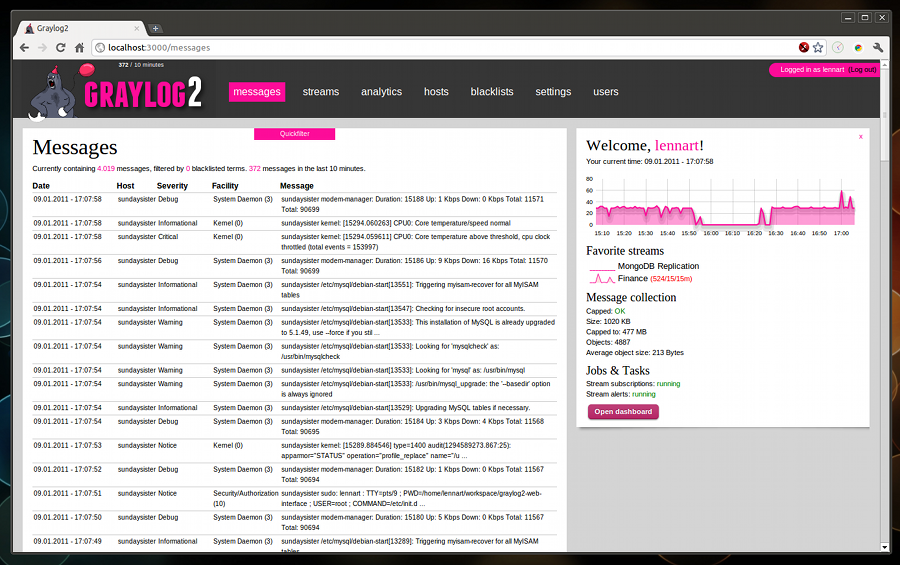
\includegraphics[scale=0.5]{assets/graylog2.png}%
		\caption[DUMMY]%
		{A GrayLog2 interfésze}%
		\label{fig:graylog2-webinterface}
\end{figure}

\Aref{fig:graylog2-webinterface} ábrán látható a GrayLog2 webes interfésze, amelynek segítségével a szakemberek könnyen észlelhetik valós időben a fennálló vagy éppen bekövetkező hibákat, továbbá kereshetnek a korábban előforduló hibákban (erre a GrayLog2 az \nomenclature{ElasticSearch}{TODO} \nomenclature{full-text search engine}{TODO} szoftvert használja) illetve könnyen beállíthatnak értesítéseket, hogy akár az éjszaka felmerülő hibákról is értesülhessen a felelős.

\section{Alkalmazás hiba monitorozás\\}
A naplózással a hibák könnyen észrevehetővé és később visszakereshető válnak, azonban a következőkre nem nyújt megoldást:\\
\begin{itemize}
\item hibák rögzítése a jegykezelő (issue kezelő) rendszerben
\item egy hiba csak egyszer kerüljön rögzítésre
\item automatikus értesítés a hibáról
\item a hibászázalék vizualizálása komponensenként
\end{itemize}

Természetesen alkalmazás hiba monitorozó rendszer nélkül is működhet rendszer jól, azonban előfordulhat, hogy nagy mennyiségű hibánál a naplógyűjtő rendszerben átsiklanak problémák felett vagy egyszerűen elfelejtésre kerülnek. A másik probléma lehet amikor a hibajelentést közvetlenül a jegykezelő rendszerbe kötik be. Ez miért lehet probléma? Egy nagy felhasználóbázissal rendelkező rendszernél, ha hiba csak a felhasználók néhány százalékánál fordul elő, akkor is szükségtelenül nagy mennyiségű jegy keletkezést fogja előidézni.\\

Az alkalmazás hiba monitorozás leginkább a nem webes alkalmazásoknál (mobil és asztali) terjedt el az utóbbi időben, ugyanis ezeknél a rendszereknél a naplók nem, vagy csak nehezen gyűjthetők valós időben.\\

Elérhető alkalmazások:
\begin{itemize}
\item Sentry - \url{http://getsentry.com}
\item Exceptional - \url{http://www.exceptional.io/}
\item Bugsense - \url{http://www.bugsense.com/}
\end{itemize}

\begin{figure}[ht]
	\centering
		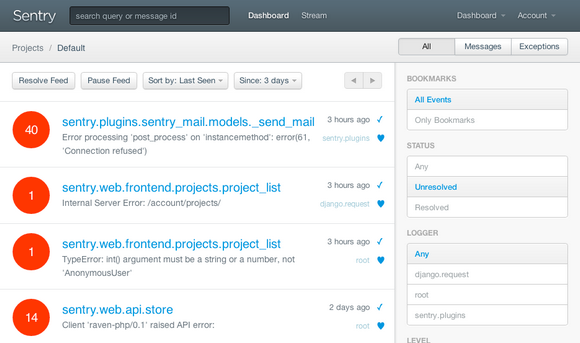
\includegraphics[scale=1]{assets/sentry.png}%
		\caption[DUMMY]%
		{A Sentry interfésze}%
		\label{fig:sentry}
\end{figure}

\section{Szolgáltatások integrálása\\}

A fejezetben említett említett szolgáltatás, szoftverek használatával a fejlesztők, adminisztrátorok már jobban megismerhetik saját alkalmazásikat, azonban ennyi felület, értesítés nyomon követése szinte már lehetetlen, ezért minden szervezet próbálja ezeket az eszközöket egymásba integrálni.
\begin{figure}[ht]
	\centering
		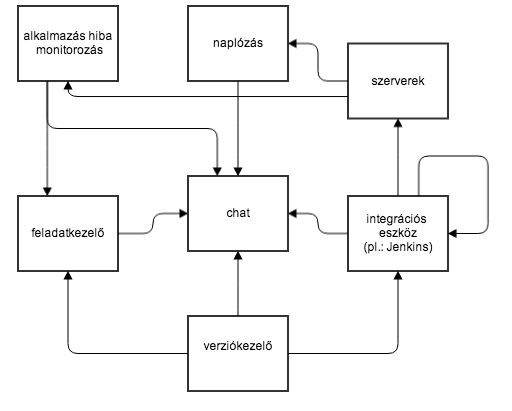
\includegraphics[scale=1.0]{assets/integrated_services.png}%
		\caption[DUMMY]%
		{A szolgáltatások egy lehetséges integrálása}%
		\label{fig:integrated-services}
\end{figure}
\Aref{fig:integrated-services} ábrán látható a szolgáltatások egy lehetséges integrációja. Első ránézésre az ábra bonyolultnak és összetettnek tűnhet, mert sok különböző egység integrációját igényli emellett a részegységeknek valós időben kell kommunikálniuk, tudniuk kell a sorrendet, és képeseknek kell lenniük egymás üzeneteinek megértésére.\\
Ezeknek az igénynek a kielégítésére minden részegység tudja, hogy kit kell neki értesítenie; az értesítések pedig ún. \emph{webhook} (\cite{web_hook}) használatával történik, amely egy egyszerű HTTP kérés, ezáltal valós időben történhet meg az következő részegység notifikálása.\\
Viszont hogyan képesek megérteni egymás üzeneteit a részegységek?\\
Erre sajnos nincs sztenderd specifikáció, azonban szinte minden említett eszköz nyílt forrású és széles körben elterjedt, ezért egymás üzeneteinek feldolgozása, megértése már megoldott beépülők használatával.\\

\Aref{fig:integrated-services} ábrán felrajzolt folyamatnak az első szintje az amikor a kód bekerül a verziókezelőbe, amely össze van kapcsolva a feladatkezelővel, ahol akár a kapcsoló jegy lezárásra is kerülhet a kód mellé csatolt üzenet szövege (\nomenclature{commit message}{TODO}) alapján, majd a chaten keresztül értesülhetnek a csapat tagjai, a projektmenedzser vagy az adott szervezeten belül bárki, aki érintett lehet az adott funkció, szolgáltatás fejlesztésében.\\
A verziókezelő másik kapcsolata az integrációs eszközzel van, amely lefuttat különböző ellenőrző, tesztelési és riportálási feladatokat, amelyek garantálják, hogy az új kódsorok megfelelnek a céges előírásoknak, nem okoznak problémát az alkalmazás futtatásában, a folyamat végén értesítést küldhet a közös chatbe az integráció sikerességéről, hiba esetén értesítheti a megfelelő személyeket, ugyanis a hiba kijavításáig senki tud hibámentes kódot beküldeni az integrációs folyamatba, ezért ennek az értesíthet a legmagasabb prioritással kell történnie. Az integrációs folyamat kimenete lehetséges, hogy újabb integrációs folyamat bemenete lesz; ez olyankor fordulhat elő, amikor az alkalmazás egyik ága egy másik ágba kerül beolvasztásra. Ez történhet például a fejlesztői ág tesztelői ágba való automatikus vagy félautomatikus olvasztásakor, vagy a minőségbiztosítási csapat (\nomenclature{QA team}{TODO}) tesztelői ág jóváhagyásaként a produkciós ágba való olvasztáskor.\\
\hfill\\
\Aref{fig:integrated-services} ábrán továbbhaladva az integrációs eszköz után az alkalmazás felhasználói elfogadási szerver (user acceptance test server) vagy előnézeti (staging, preview) szerverre kerül, amely egy homokozószerű, zárt, a produkciós szerverrel megegyező architektúrájú környezetben nyújt lehetőséget az alkalmazás tesztelésére. Majd ezután kerülhet ki a produkciós szerverre. Mind a felhasználói elfogadási, az előnézeti és a produkciós szerverek hibáit már naplózni illetve az ezeken futó alkalmazásokét is; hiba esetén pedig értesíteni kell a chaten keresztül az hibát okozó komponens, vagy alkalmazás részért felelős személyt, csapatot. A felelősök a hibáról hibajegyet készíthetnek a feladatkezelőbe, majd a fejlesztőcsapatok javítva a hibát a kódot beküldik a verziókezelőbe és a folyamat újraindul.\\
\hfill\\
Fontos felhívni a figyelmet, hogy \aref{fig:integrated-services} ábrán rendkívül komoly hangsúlyt kapott a chat rendszer, természeten nem kötelező csetet használni, azonban a valós idejű értesítésekre illetve a reakcióidő csökkentése érdekében mindenképpen ajánlott. Továbbá az ábrán nem szerepel, de a cset alapú notifikálás mellett érdemes egy értesítése formákat is használni, mint például az email, vagy magas prioritású hibáknál (alkalmazásleállás) érdemes lehet megfontolni az sms, okostelefon valós idejű üzenet (\nomenclature{Push Notification}{TODO}), esetleg csipogó használatát.

\subsection{Hubot}
Ha egy szervezet úgy dönt, hogy csetet fog használni a rendszerek, alkalmazások valós idejű követésére, akkor találkozni fog a következő problémákkal:
\begin{description}
\item[Rendszerautomatizáció] hiába automatizált a folyamat, ha az egy-egy pontról történő elindítás nem lehetséges, bárhonnan, bármikor.\\
Ilyen probléma lehet az integrációs rendszer elindítása a kód egy pillanatnyi állapotától kód beküldés nélkül.
\item[Távoli irányítás] lehet, hogy egy asztali számítógépen könnyen elvégezhető a produkciós rendszeren egy verzióváltás, de miért ne lehetne ezt megtenni egy okostelefonról is?
\item[Kommunikáció külső eszközök használatakor] ha egy üzenet érkezik (például alkalmazás újraindítás szükségességéről), akkor a csapat tagjainak meg kell beszélniük, hogy ki javítja meg a problémát.
\end{description}
GitHub, Inc., wrote the first version of Hubot to automate our company chat room. Hubot knew how to deploy the site, automate a lot of tasks, and be a source of fun in the company. Eventually he grew to become a formidable force in GitHub. But he led a private, messy life. So we rewrote him.

Today's version of Hubot is open source, written in CoffeeScript on Node.js, and easily deployed on platforms like Heroku. More importantly, Hubot is a standardized way to share scripts between everyone's robots.

\chapter{DevOps}
%!TEX root = /Users/oroce/Documents/msc-szakdolgozat/dolgozat.tex

Az informatikai fejlesztések evolúciójának köszönhetően megszületett agilis irányzatok (agilis fejlesztés, scrum, kanban irány, extrém programming) megszüntették a klasszikus funkcionális csapatokfelépítést, ennek a következő iterációja a DevOps irányzat, amely a fejlesztés (\textbf{Dev}elopment) és az üzemeltetés (\textbf{Op}erations) szavaknak a keresztezéséből született meg.

\section{Kialakulása}

\brparagraph{Keresztfunkciós és termékcsapatok}
A keresztfunkciós (cross-functional) csapatok és termékcsapatok létrejöttével az egy-egy funkcióra specializálódott csapatok (minőségbiztosítás, frontend, middleware, backend csapatok) felbomlottak és kész szolgáltatások fejlesztésére rendezkedtek be. A szolgáltatást nyújthatják akár cégen belül, akár cégen kívül, de a csapat felelőssége a következőkre terjed ki:
\begin{itemize}
  \item tervezés
  \item megvalósítás
  \item tesztelés
  \item dokumentálás
  \item élesítés
  \item monitorozás
  \item kiértékelés
  \item marketing
\end{itemize}
Így pedig a fejlesztés és az üzemeltetés szétválasztása a szervezet méretétől függetlenül a csapat méretét figyelembe véve túl költséges lenne.

\brparagraph{A felhőalapú szolgáltatások}
A felhőalapú szolgáltatások előretörésével, az infrastruktúra alapú (\nomenclature{IaaS}{Infrastructure as a Service a felhő alapú szolgáltatások egy olyan típusa, amelyben nem egy konkrét kerül értékesítésre, hanem a számítási kapacitás egy virtualizált környezetben. A legismertebb ilyen szolgáltatók az Amazon Web Services, Joyent és Google Cloud.}) szolgáltatások tekintetében valamelyest, de a platform alapúaknál (\nomenclature{PaaS}{Platform as a Service a felhőszolgáltatások egy típusa, amely a számítási kapacitáson túl a szoftverkomponensek futtatására már elő van készítve, azaz az infrastruktúra kiépítése és karbantartása a szolgáltatás része. A leggyakrabban használt PaaS szolgáltatók az AWS Beanstalk, Heroku.}) teljességgel kijelenthető, hogy az üzemeltetési feladatok csökkennek és egy kisebb csapatban nincs szükség dedikált személyre. Természetesen ez nem jelenti, hogy kevesebb a feladat, csupán a feladatok alakulnak át, hiszen egy-egy számítási egység megfeleltethető egy-egy alkalmazásnak, amelynek köszönhetően a hosztok provizionálása szükségtelen, csupán az alkalmazások provizionálására van szükség.

\brparagraph{Transzparencia a fejlesztés és az üzemeltetés területén}
\begin{quote}
DevOps is the practice of operations and development engineers participating together in the entire service lifecycle, from design through the development process to production support.
\end{quote}
\begin{flushright}
\citet*{agile_admin}
\end{flushright}

Mueller megfogalmazása alapján könnyen belátható, hogy a fejlesztők és az üzemeltetés feladatai gyakran összekapcsolódnak, kiegészítik, fedik egymást, tehát érdemes szervezeti szinten is jelezni a két feladatkör kapcsolatát a DevOps feladatkör használatával.
Továbbá a két munkakör mélyebb integrációjával a fejlesztés állapotai (development, staging, production) érthetőbbé válnak az érintettek számára, ugyanis míg az üzemeltetés a fejlesztés első lépéseit nem látja, így automatizálni, optimalizálni sem tudja, illetve közvetlenül nem tud segítséget nyújtani az új eszközök kiválasztásában, addig a fejlesztők az éles környezetben felmerülő problémákkal nincsenek tisztában. Viszont ha az üzemeltetés részt vesz a fejlesztésben, megérthetik az egy-egy funkció mögött rejlő döntéséket, megismerhetik az alkalmazás gyenge pontjait és hiba esetén sokkal hamarabb tudják lokalizálni a problémát vagy akár még a fejlesztési szakaszban kijavításra kerülhet a hiba. A fejlesztők megérthetik az infrastruktúra határait, a konfiguráció menedzsmentet és mindezek hatásait az alkalmazásra.\\
A DevOps irányzat akkor tud a legsikeresebb lenni, ha a szervezet illetve a szervezet tagjai nem egy új szereplőként tekintenek rá hanem a szervezeti kultúrába integrálják, az ugyanis nem más mint a tudásmegosztásnak egy olyan formája, amely mind az egyéni-, mind a szervezeti érdekeket is szolgálja.

\section{Szerepe}

A DevOps munkakör szerepe a visszajelzések felgyorsulásával párhuzamosan került elő. \Aref{chap:cont_int} fejezetben bemutatásra került a folyamatos integráció, a tesztvezérelt fejlesztés fontossága, amelyek sokkal mélyebb architekturális tudást feltételeznek, mint amire egy klasszikus programozónak szükséges van. De ez szintén igaz, \aref{chap:cont_not} fejezetben bemutatott folyamatos értesítésekre is, hiszen az szoftver folyamatosan tesztelve van, folyamatosan naplóbejegyzéseket küld, melyeknek a megértéséhez az egész rendszert felépítésével kell tisztában lenni. Természetesen ez a fajta munkakör kialakulása amellett, hogy egyesíti a fejlesztők és a üzemeltetők tudását és ahhoz vezet, hogy a felelősségi körük is összeadódik.\\
Míg a megnövekedett felelősség távol tarthatja a szervezet tagjait a DevOps munkakörtől, addig mind a szoftver, mind a szervezet nagyon sokat tanulhat és profitálhat az egyesített munkakör okozta horizontális látásmódtól.

\brparagraph{Konfiguráció menedzsment}
A konfiguráció menedzsment, illetve az automatizálás a DevOps munkakör leggyakrabban emlegett előnyei. Mivel a DevOps szakemberek mind a fejlesztési-, mind a tesztelési, mind a produkciós környezetben felmerülő problémákkal tisztában vannak, viszont különböző környezetekben megszerzett tudásukat könnyen át tudják transzformálni egy másik környezetre, ezért olyan pontokon is tudnak automatizálást végezni, mely nagyban növelheti a hatékonyságot és magabiztosáságot. Ilyen például a környezetfüggetlen konfiguráció menedzsment, mely a fejlesztési környezetben munkát végzők napi rutinjait egyszerűsíti és a tesztelési lehetőségeiket növeli.

\brparagraph{Incidens menedzsment}
Az incidensek kezelése mindig nehéz dolog, főleg olyan esetekben, amikor nehéz meghatározni, hogy a szoftverrendszer mely részegysége okozza problémát. A probléma megoldása akkor tud főleg elhúzódni, ha az incidens kezelő rendelkezik vakfoltokkal a rendszert illetően ezért a hiba lokalizálása is problémát okoz. Viszont a rendszer részegységeivel, mind a működtetett kóddal tisztában lévő emberhez kerül egy incidens nagyobb valószínűséggel fogja a hibát okát megtalálni, és akár ki is javítani.

\brparagraph{Jobban integrált folyamatok}
Mivel a klasszikus üzemeltetés nem igényel részvételt a egy-egy termékcsapat életében, ezért a termékcsapatok olyan eszközökhöz nyúlhatnak, amelyek működtetése az üzemeltetés számára ismeretlen, amely konfliktusforrás lehet a két érintett csoport között. Viszont ha kiválasztási folyamatban szereplők dolgoznak üzemeltetésen és termékcsapatban is, a szoftverkomponens cégen belüli bevezetése könnyebb lesz.

\chapter{ChatOps}
\label{chapter:chatops}
%!TEX root = ./dolgozat.tex

Jelen dolgozat tárgyalja annak szükségességét, hogy az alkalmazás integritása állandóan tesztelve legyen (continuous integration), melynek segítségével a szervezet tagjai állandóan visszajelzést kaphatnak az éppen folyamatban lévő fejlesztések, javítások állapotáról. Továbbá a DevOps irány az, amellyel a visszajelzés, a hibajavítás és önmagában a reakcióidő csökkenthető. A keresztfunkciós csapatok meglétével a csapatok horizontális skálázása is lehetővé válik. Az viszont nem került tisztázásra, hogy mindezek hogyan kapcsolódnak össze, hogy válnak valójában elérhetővé és miképpen lehet rájuk minél gyorsabban, transzparensebben reagálni. Ez a fejezet erre hivatott válaszolni, mégpedig a ChatOps irányzattal, amely az angol Chat (beszélgetés) és Ops (operations, üzemeltetés) szavak összevonásából keletkezett.

\section{Kialakulása}

Mind a ChatOps név, mind pedig az első implementáció a GitHub cégnek köszönhető. A cég indulása idején 2006-ban már minden kommunikáció az egyik népszerű chat szolgáltatás segítségével (Campfire) történt. A cég növekedésével párhuzamosan egyre több információra volt szükség egy-egy csapatnak a többi csapattól, illetve az üzleti elemzők, a marketing adatigénye azt okozta, hogy a chaten folyamatosan írtak a fejlesztőknek és az adatbázis hozzáféréssel rendelkező kollégáknak az igényükkel, amelyet a termék fejlődése érdekét szem előtt tartva kielégítették (\cite{what_is_chatops_slideshow}). Ez az adatigénylés gyakran csak arra vonatkozott, hogy működik-e a weboldal éppen Japánban, sikerült-e élesíteni a kereséshez kapcsoló hibákat vagy hány fizető felhasználó használta a weboldalt ez előző napon. Ez azt eredményezte, hogy megpróbálták a fejlesztők automatizálni az adatexportálást, azonban ezt nem ad-hoc szkriptekkel tették meg, hanem egy robottal, ami figyel a chaten történő beszélgetésekre és tud rájuk reagálni. Ennek az iránynak több előnye is volt, ugyanis az első adatigénylés után a lekérdezés automatizálásra került, a robot már végre tudta hajtani a lekérdezést, így a fejlesztő kiadta először a parancsot, amelynek hatására a kívánt eredmény láthatóvá vált azonnal chaten. Mindezt látta az is, akinek az információra szüksége volt, így amikor legközelebb ismét felmerült az adatigénye, már nem kellett mások segítségét igénybe venni, hiszen ő maga is végre tudta hajtani az utasítást. \Aref{fig:pager_sup} ábrán látható, ahogy a Campfire chatrendszerben lekérdezésre kerül az incidensek állapota. A robot válasza azt jelenti, hogy jelenleg nincs incidens, tehát minden rendszer megfelelően működik. \\
A másik fontos irány, ami megalapozta a ChatOps létrejöttét az maga az Ops része a szónak, vagyis az üzemeltetés. A GitHub már kezdetek óta a DevOps filozófiát követi, amelynek köszönhetően egy-egy termékeket több csapat is fejleszt, a csapatok tagjai folyamatosan fluktuálódnak, keverednek.  2014-ben egy átlagos héten a fő terméken 67 ember dolgozott (\cite{github_product_team}), amely azt jelenti, hogy a hét bármely időszakában legalább 67 ember állíthatta élesbe a terméket, ugyanis nem csak teljesen kész fejlesztések kerülhetnek élesítésre, köszönhetően a GitHub által is aktívan alkalmazott funkciókapcsolóknak (feature flag)\nomenclature{funkciókapcsoló (feature flag)}{\hfill\\Az élesítésnek egy olyan formája, amely során a funkció élesítésre kerül produkciós környezetbe, viszont csak a kiválasztott felhasználók számára. A kapcsoló használata bevált módszer a kísérleti, félkész, validálás alatt álló funkciók bevezetésére.} köszönhetően (\cite{github_feature_flag}). Ahhoz viszont, hogy bárki bármikor élesíthessen egy kész vagy akár csak prototípus szintjén lévő fejlesztést, teljes transzparencia szükséges, minden résztvevőnek látnia kell, hogy éppen valaki élesít vagy valaki már foglalkozik egy élesítés okozta problémával.\\
\Aref{fig:hubot_deploy} ábrán látható, ahogy az élesítés utasítás kiadásra kerül. A jelen esetben egy speciális verziója a kódnak (smoke-perf) az éles szerverek egy részére (fe1) kerül ki, ez a chatben mindenki számára látható és egyértelmű, hiszen csak angol nyelvű kifejezések kerülnek használatra a robot vezérlésére.

\begin{figure}[H]
  \centering
    
\includegraphics[scale=1.4]{assets/pager_sup.jpg}%
    \caption[DUMMY]%
    {Incidensek lekérdezése Hubot segítségével, forrás: \cite[p.~83]{what_is_chatops_slideshow}}%
    \label{fig:pager_sup}
\end{figure}

\Aref{fig:hubot_status} ábrán viszont már látható, amint egy elrontott élesítés után értesíteni kell az érintetteket, arról hogy a művelet sikertelen volt, ezért vissza kell vonni. Ennek a parancsnak a nagyszerűsége az, hogy nem csak a chaten aktív emberek látják, hanem frissíti a szolgáltatás publikus státusz oldalát is (\url{https://status.github.com}).

\begin{figure}[H]
  \centering
  \begin{minipage}{.45\textwidth}
    \centering
    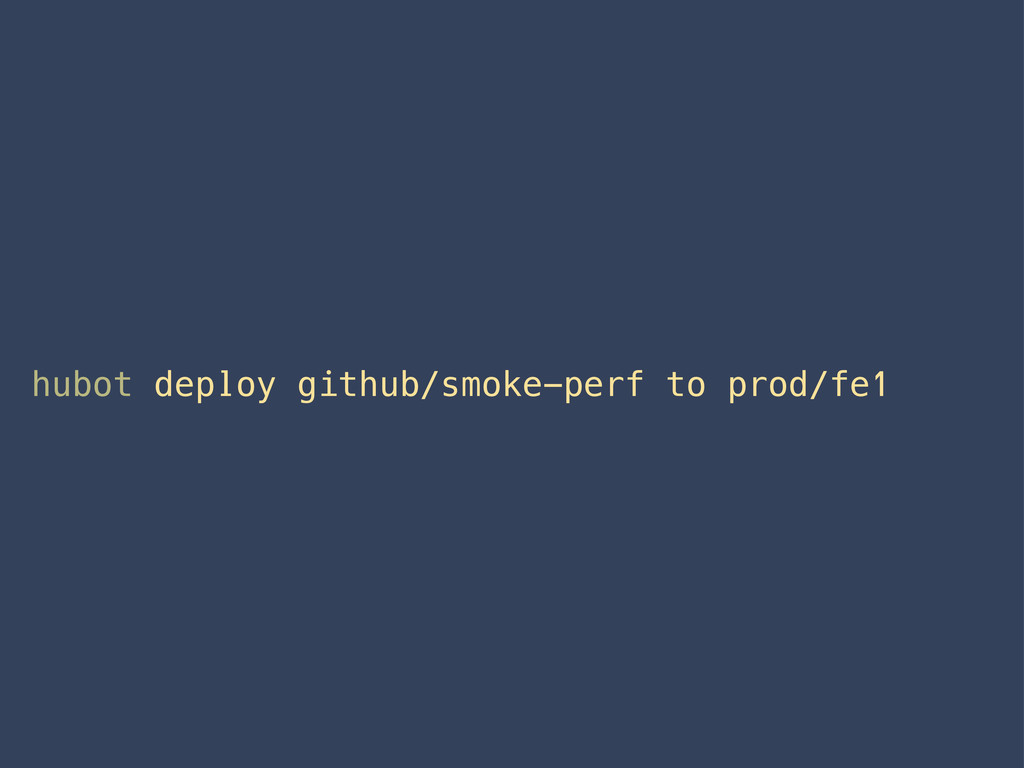
\includegraphics[scale=0.90]{assets/hubot_deploy.jpg}%%
    \caption[DUMMY]%
    {Élesítés robot segítségével,\\forrás: \cite[p.~40]{what_is_chatops_slideshow}}%
    \label{fig:hubot_deploy}
  \end{minipage}\hfill
  \begin{minipage}{.45\textwidth}
    \centering
    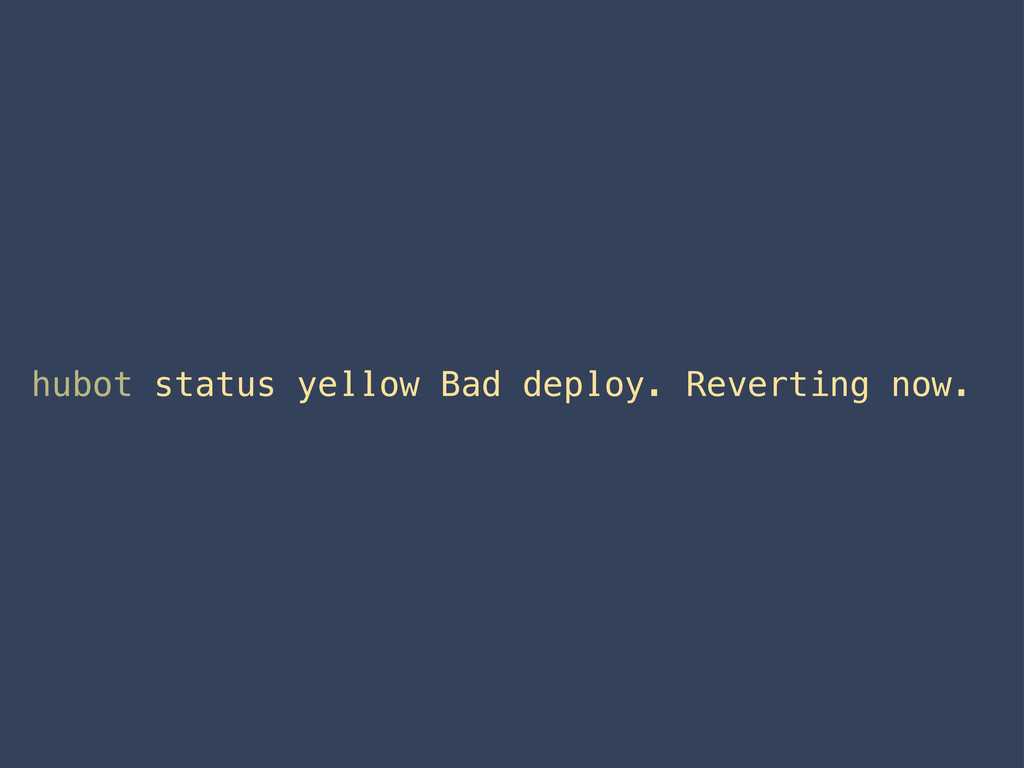
\includegraphics[scale=0.90]{assets/hubot_status.jpg}%
    \caption[DUMMY]%
    {Értesítés rossz élesítésről,\\forrás: \cite[p.~48]{what_is_chatops_slideshow}}%
    \label{fig:hubot_status}
  \end{minipage}\hfill
\end{figure}

\brparagraph{Robot szerepe}
A chatrendszerbe a robot úgy csatlakozik, ahogyan egy ember is tenné, minden üzenet megérkezik hozzá és ezekre reagál. A robot önmagában nem tartalmaz üzleti logikát, mindössze a felhasználók üzenetei alapján képes a programozható interfészekhez (API) hívásokat intézni.

\section{Tulajdonságai}

\brparagraph{Jobb kommunikáció}
\label{subsection:better_communication}
Egy csapatban sok különböző szereplő lehet, amennyiben a csapat agilisan fejleszt, akkor feltehetően lesznek technikai és nem technikai emberek, akik annak ellenére, hogy egy 5-6 fős csapatban dolgoznak, differenciált információval és tudással rendelkeznek a terméket illetően. Egy nagyon egyszerű példa, ha a csapat egy olyan termékért felelős, amelyért lehet fizetni, viszont a fizetési szolgáltatás egy hibája, mérhető csökkenést fog okozni a csapat által fejlesztett szoftver mérőszámai alapján. Azonban egy másik szolgáltatás vagy szoftverkomponens állapota könnyen ellenőrizhető egy ChatOps alapú szervezetben, \aref{fig:get_outage_for_payment} példa ezt hivatott bemutatni.\\

\begin{figure}[H]
    \begin{alltt}
    @hubot incident? for payment on last week
    \end{alltt}
    \caption[DUMMY]%
    {Az előző heti incidensek listázása a fizetési rendszerhez}%
    \label{fig:get_outage_for_payment}
\end{figure}

Egy másik gyakran előforduló problémát jelentenek az éjszakai leállások, amikor az ügyeletes akár reggelig a probléma javításán dolgozott és reggel még munkaidő kezdetére nem ért be, akkor könnyen látható, hogy meddig próbálta megjavítani a hibás részt illetve, hogy mit tett a javítás elvégzése érdekében.

\brparagraph{Transzparens}

Az előző pontban kifejtett okok is részben a transzparenciát segítik elő, de a chat rendszer használata már önállóan segíti az átláthatóságot.
Egy szervezet általában sok formáját használja a kommunikációnak:

\begin{itemize}
  \item szöveges üzenetek
  \item tennivalók listája / issue kezelő rendszerek
  \item hibabejelentő rendszerek
  \item telefonhívások
  \item videóhívások
  \item email
  \item sárga cetli
\end{itemize}

Azonban a sok eszköznek köszönhetően biztosan kimaradnak olyan érintettek, akiknek szükségük lenne információra, viszont ha mindezt egy könnyen elérhető felületen keresztül centralizálják, akkor mindenki számára könnyebbé válik az információhoz való hozzáférés.\\
\Aref{lst:search_feature_call} példa kívánja bemutatni, hogy a chat, mint munkaszervezési platform miért tud jól működni. Ha a példában látható Joey és Paul a beszélgetést telefonon vagy emailben ejti meg, akkor Bill semmiképp sem tudott volna csatlakozni a beszélgetéshez, és az implementáció csak egy későbbi szakaszában derült volna fény a Bill által említett problémára.

\begin{figure}[H]
  \begin{alltt}
Joey: @coworker2: We should talk about the new search feature!
Paul: Sure, a quick videocall?
Joey: Sure
Paul: hubot videocall
hubot: Click here to join the video call
       http://videocall.me/conversation/8046741f-1d67
Bill: hey @Joey, @Paul I will join too because I'm going to implement it 
      and there are a few things in the specification which won't work :(
  \end{alltt}
  \caption[DUMMY]%
    {Egy elképzelt beszélgetés, mely jól személteti, hogy a beszélgetéshez, amely elvileg csak Paul és Joey között zajlott volna, még csatlakozott Bill is}%
    \label{lst:search_feature_call}
\end{figure}

Természetesen a centralizálás nem azt jelenti, hogy minden beszélgetést a chaten kell megejteni, hiszen felesleges lenne ennyire központosítani mindent és előbb vagy utóbb feltehetően munkavállalói ellenállásnak köszönhetően csökkenne a chat használata. Továbbgondolva \aref{lst:search_feature_call} példát, a videóbeszélgetés ugyan nem elérhető chaten, viszont a beszélgetés arról, hogy a keresés működésének megbeszélése videóbeszélgetés formájában történt meg az igen, illetve ehhez hasonlóan elérhető a videóbeszélgetéshez tartozó link is elérhető (amihez használt szoftver valószínűleg támogatja a videóbeszélgetések rögzítését). A példa jól vizualizálja a chat alapú munkavégzés legnagyobb előnyeit: a kronológikus áttekinthetőséget, a korábbi beszélgetések kereshetőséget, bár ez igaz az emailekre is, viszont itt egy csapat minden tagja megtekintheti, nem csak azok, akik rajta voltak a címzett listán.\\

\brparagraph{Egy interfész}
A legtöbb szervezet életében időről időre kerülnek bevezetésre új szoftverek, amelyek betanítási folyamatot igényelnek. Ráadásul, ha nehezen illeszkednek a szervezeti kultúrába, akkor gyakran a munkavállalók ellenségesen állhatnak a bevezetéssel szemben. Egy nagyon egyszerű példán lehetne ezt szemléltetni, ha be szeretne vezetni a szervezet egy munkaidő nyilvántartó szoftvert, akkor annak a kitöltéséhez feltehetően a következő lépéseket kellene végrehajtani:

\begin{description}
  \item[Autentikáció]\hfill\\
  Amennyiben az adott szoftver támogatja, illeszkednie kell a szervezet authenkációjához (LDAP, OpenID), amennyiben ez nem lehetséges abban az esetben a felhasználóknak egy újabb jelszót is meg kell jegyezniük, amely bizonyára nem fogja gyorsítani a bevezetést.
  \item[Érkezés vagy távozás kiválasztása]\hfill\\
  Az érkezés vagy távozás kiválasztása.
  \item[Idő rögzítése]\hfill\\
  Az érkezési vagy távozási idő megadása, esetleg további egyéb megjegyzés kíséretében.
  \item[Kijelentkezés]\hfill\\
  Az alkalmazásból történő kijelentkezés a művelet elvégezése után.
\end{description}
\hfill\\
Ezzel szemben \aref{lst:workhour_with_hubot} ábrán látható egy elképzelt munkaidő nyilvántartás robot segítségével chaten keresztül történő rögzítéssel. Könnyen belátható, hogy a robottal történő adminisztrálás sokkal gyorsabb és egyszerűbb, mint egy különálló felületen keresztül.

\begin{figure}[H]
  \begin{alltt}
Bill (08:32): hubot arrived
...
Bill (17:34): hubot leaving for my daughter's violin concert
  \end{alltt}
  \caption[DUMMY]%
    {Munkaidő nyilvántartás chaten keresztül robottal}%
    \label{lst:workhour_with_hubot}
\end{figure}

Természetesen ennek a bevezetése is sokáig eltarthat, hiszen lehet, hogy a szervezet tagjai chaten sem fogják elküldeni az üzenetet a robotnak arról, hogy megérkeztek, mint ahogy a célszoftverbe se lépnének be. Azonban a be nem jelentkezett felhasználókat a szoftver esetleg email utján tudja értesíteni vagy a felettesüket tudja tájékoztatni, addig a robot sokkal jobb felhasználói élmény biztosítása mellett képes ezt megtenni. \Aref{lst:workhour_with_hubot_ux} ábrán ezt lehet megtekinteni. Mivel a chat a kommunikáció központi forrása, ezért a robotnak egyszerűen a felhasználók cselekvéseit kell figyelemmel követnie és azokra reagálnia.

\begin{figure}[H]
  \begin{alltt}
Steve (08:32): <answering question>
Steve (08:35): <asking question>
Steve (08:43): <answering question>
Steve (09:02): <answering question>
hubot (09:02): Hey @Steve it seems you've been here for 30 minutes
               but you haven't checked in yet, shall you?
Steve (09:02): hubot arrived at 08:32
    \end{alltt}
    \caption[DUMMY]%
    {A munkaidő nyilvántartás bevezetése sokkal felhasználóbarátabb tud lenni egy robot segítségével}%
    \label{lst:workhour_with_hubot_ux}
\end{figure}

Ezen túl egyre több szervezetben a szervezet tagjai már nem csak asztali eszközökön kapcsolódnak az internetre, hanem több eszközről. Ilyen például a BYOD (Bring Your Own Device)\nomenclature{BYOD (Bring Your Own Device)}{\hfill\\Olyan vállalati szabályozás, amely megengedni, hogy a szervezet tagjai a saját eszközeiket használják a vállalati adatok és rendszerek eléréséhez. Mivel a munkavállalók a céges szabályok ellenére is magukkal viszik az eszközeiket, ezért inkább támogatják a használatukat, ahelyett hogy korlátoznák.} irányzat, amellyel azokat a céges szabályokat illetik, melyek megengedik, hogy a munkavállalók saját személyes eszközeiket használják a munkavégzéshez, ez lehet:

\begin{itemize}
  \item asztali számítógép
  \item notebook
  \item mobiltelefon
  \item okosóra
  \item tablet
  \item könyvolvasó
\end{itemize}

A lista hosszának csak a képzelet, illetve az elérhető internetképes eszközök számossága szab határt. Ezt a számot csak többszörözi az a tény, hogy ezek az eszközök különböző operációs rendszerek különböző verzióit futtatják. Ezek alapján is könnyen belátható, hogy mennyivel egyszerűbb egy szöveges kommunikációra szakosodott chat rendszert használni, mint egy saját felhasználói interfésszel rendelkező rendszert bevezetni, amely feltehetően nem is fogja támogatni az elérhető eszközök töredékét sem.\\
\newline
Természetesen nem minden szoftver helyettesíthető mindössze egy pár szöveges utasítással, azonban érdemes belegondolni, hogy sok kis adminisztrációs rendszer sokkal felhasználóbarátabb és akár erőforrástakarékosabb lenne, ha csupán néhány parancs kiadásával lehetne irányítani ahelyett, hogy egy komplex felületen keresztül lehet őket elérni, amely ráadásul csak az asztali gépen meghatározott böngészőből érhető el.

\brparagraph{Absztrakció}
Az absztrakció építése mindig költséges, de a szervezet jövőbeni lehetőségeit nagyban növeli, ha a fent említett munkaidőszervezési példánál maradva a szervezet a külső szoftver mellett dönt. Ha azonban egy év után arra a döntésre jut a szervezet, hogy a munkaidőnyilvántartás szükséges és a használt szoftvert lecseréli egy jobb piaci ajánlatnak köszönhetően, akkor számolnia kell a munkavállalókban keltett, újabb szoftver bevezetése okozta frusztrációval.\\
Ha viszont a munkaidőnyilvántartás chaten keresztül kerül megoldásra, a háttérben lévő implementáció vagy szoftver könnyen cserélhető, hiszen a dolgozók előtt rejtve volt eddig is, ezért nem is fogják észrevenni, hogy mi történt a háttérben (a használatához szükséges parancsok módosítást nem igényelnek).

\brparagraph{Aszinkron kommunikáció}

A kommunikációt két részre lehet tagolni a résztvevő felek időbeosztása alapján: szinkron és aszinkron. A szinkron kommunikáció során a résztvevő feleknek az időbeosztása meg kell, hogy egyezzen, azaz az egyik résztvevő fél kérdésére a másik résztvevő fél azonnal válaszol, tehát a válasz megérkezésének késésétől el lehet tekinteni, azaz nullának tekinthető. A kérdező résztvevő azonnali válaszadásra számít a válaszoló részéről, így működik a szóbeli beszélgetés.\\
Ezzel ellentétben az aszinkron kommunikáció során a résztvevő felek nem számítanak azonnali reakcióra, ilyen kommunikációra példa az email, amely elküldése után a küldő tisztában van vele, hogy a válasz megérkezése és az elküldés között eltelt idő több mint nulla lesz.\\
\newline
Szinkron kommunikáció jellemzői:

\begin{itemize}
  \item a résztvevő felek időben egyszerre vesznek részt a kommunikációban
  \item gyors módja a kommunikációnak
  \item rövid reakcióidő
  \item erős egymásrautaltság
  \item nagy információáramlás
  \item párhuzamosan csak egy kommunikációban lehet részt venni
  \item jellemző típusai:
  \begin{itemize}
    \item személyes találkozás (több ember esetén megbeszélés)
    \item hívás (videó, hang)
  \end{itemize}
\end{itemize}
A szinkron kommunikáció jellemzően gyors, pörgős, információgazdag, viszont cserébe nagy koncentrációt igényel az idő egy bizonyos pontjától (kommunikáció kezdete) egy másik pontjáig (kommunikáció vége). Egy szervezet esetében ezek a meetingek, szemtől szembe lezajló beszélgetések, brainstorming vagy akár videó- vagy audióhívások lehetnek; egyetemen a tanórák, a csoportos projektfeladatok jó példák a szinkron kommunikációra.\\
\newline
Aszinkron kommunikáció jellemzői:
\begin{itemize}
  \item a résztvevő felek eltérő időben vesznek részt a kommunikációban
  \item lassú módja a kommunikációnak
  \item hosszú reakcióidő
  \item párhuzamosan több kommunikációban is részt lehet venni
  \item elosztott kommunikáció
  \item közvetett egymásrautaltság
  \item alacsonyabb szintű információáramlás
  \item jellemző típusai:
  \begin{itemize}
    \item email
    \item SMS
    \item chat üzenet
    \item levél
  \end{itemize}
\end{itemize}

Az aszinkron kommunikáció jóval lassabb, mint a szinkron, viszont időben nincsenek a résztvevők megkötve, amely természetesen azt jelenti, hogy a reakcióidő megnőhet, illetve lassabb lehet a kommunikáció, csökkenhet a hordozott információmennyiség.\\
\newline
Az előző felsorolás alapján könnyen látható, hogy a szinkron kommunikáció sokkal hatékonyabb és gyorsabb, mint aszinkron társa, azonban sok esetben a szinkron nem megvalósítható, illetve nagyobb erőforrásigénnyel rendelkezik, mint az aszikron. A következő példák ezt kívánják bemutatni:

\begin{description}
  \item [Földrajzilag elosztott csapatok esetén] \hfill\\
  Földrajzilag elosztott csapatok vagy csak ideiglesen eltérő időzónában lévő csapatok esetében a szinkron kommunikáció gyakran nem lehetséges, hiszen többórás időeltolódás esetén a munkavégzést megnehezíti, ha egymásra kell várni.
  \item [Más feladat végzése közben] \hfill\\
  A szinkron kommunikáció hatékonyságával vetekedni valóban nem lehet, viszont a szinkron kommunikáció azt jelenti, hogy a kommunikáció megkezdésekor végzett feladatot meg kell szakítani (legalább ideiglenesen), majd a kommunikáció végeztével lehet folytatni a korábban végzett feladatot, amely könnyen belátható, hogy sok megszakításnál a feladat el nem végzésébe torkollhat.
  \item [Információ hiányában] \hfill\\
  Amennyiben a kommunikációt kezdeményező félnek a kérdésére vagy adatigénylésére a válasz hosszabb ideig tart, ez lehet akár pár perc, óra, napok vagy hónapok, akkor az aszinkron kommunikációnak nincs alternatívája. 
\end{description}

Minden feladat nem rendezhető csak szinkron vagy aszinkron csoportba, ezért érdemes a két kommunikációs formát keverni és egy megfelelő mixet kialakítani, amelyet hozzá lehet illeszteni a szervezeti kultúrához. A túlzásba vitt szinkron kommunikáció azt jelenti, hogy a szervezet rengeteget fog kommunikálni, viszont a feladatok nem lesznek elvégezve a sok megszakításnak köszönhetően. Amennyiben az aszinkron irány erősödik meg, akkor a döntések meghozatala fog lelassulni vagy információhiányos állapotban kerülnek a döntések meghozatalra.

Ha a szervezeten belüli szinkron kommunikációt (telefonhívás, videóhívások) sikerül minimalizálni, akkor lehet növelni a szervezet tagjainak terhelhetőségét és minimalizálni az állandó kontextusváltás okozta frusztrációt, miközben minden kérdés és válasz dokumentálásra kerül a chatrendszernek köszönhetően.

\brparagraph{Tanulva végzett munka - Learning by Doing}
A szervezet felépítésének, mindennapjainak komplexitását jól szemlélteti egy új tag belépése a szervezetbe, akinek meg kell mutatni a munkavégzést. Ezt követketően -az egyedüli használat során- rutin műveletté kell transzformálnia azt, ez mindenki számára nagy stresszor. Hasonlóan problémás lehet, mint a már korábban említett új szoftver bevezetése. Ott bemutatásra is került, hogy miért felhasználóbarátabb egy szöveges üzenetekkel elérhető szoftver.

\begin{figure}[H]
  \centering
    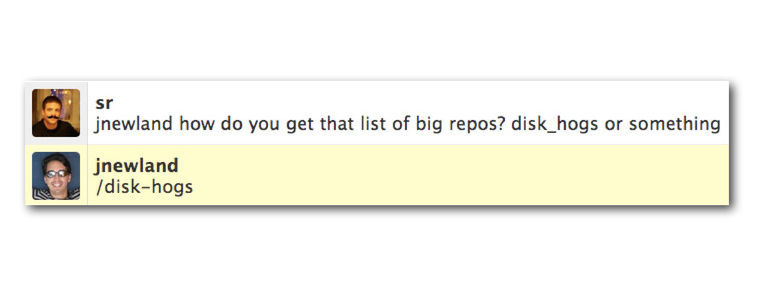
\includegraphics[scale=.6]{assets/github_disk_how_is_it.png}%
    \caption[DUMMY]%
    {Tanulás kommunikáció közben, forrás: \cite[p.~65]{what_is_chatops_slideshow}}%
    \label{fig:learn_by_doing}
\end{figure}

\Aref{fig:learn_by_doing} képen látható beszélgetés a GitHub szervezetében kívánja bemutatni, hogyan tanulnak az emberek, miközben végzik a munkájukat. Aki nem ért valamit, kérdezhet és miközben megkapja a választ, már az eredmény is láthatóvá válik. Ha később elfelejtené, akkor bármikor visszalapozhat az első napján született beszélgetések naplójához, amikor megmutatták neki a parancs működését. Továbbá a kereső bárki számára elérhető, és mindenkinek az üzenete elérhető, ezért megnézhető, hogy ki milyen parancsokat használ egy-egy feladat elvégzésére.

\brparagraph{Incidens menedzsment új szintje}
Az incidens menedzsment egy nehéz dolog, ugyanis gyakran éjszaka kell reagálni a felbukkanó hibákra a Runbook\nomenclature{Runbook}{\hfill\\A szoftverek működtetésének és azok működése során fellépő incidensek kezelésének lépéseit tartalmazó gyűjtemény.} által meghatározott módon. A ChatOps előnyeinek felsorolása közül nem véletlen kerül utoljára tárgyalásra ez a fontos terület, ugyanis ebben egyesül a chat alapú munkavégzés legtöbb pozitív tulajdonsága.\\
Az incidensek megfelelő kezeléséhez szükségesek a következők:
\begin{itemize}
  \item kezelnie kell az incidens hibajegyét
  \item a lehető legtöbb információra van szükség a hibát illetően
  \item az ügyeletet végzőnek tudnia kell értesíteni a felelős csapatot
  \item dokumentálni kell minden elvégzett műveletet
  \item figyelni kell a metrikák (hibaszázalék, válaszidő) változását
  \item küldeni kell értesítést a státusz oldalra
  \item követni kell a Runbook utasításait
  \item ha nem sikerül elhárítani a hibát az ügyelet lejártáig, tájékoztatni kell a következő ügyeletest
\end{itemize}
\hfill\\
\begin{figure}[H]
  \begin{alltt}
hubot (1:12): Failure detected in frontend, alert created with id 1337:
              http://yourduty.com/incident/frontend/1337, @Brian has 
              been alerted
Brian (1:12): hubot pager ack 1337
hubot (1:13): \emph{Incident 1337 has been acknowledged by Brian}
Brian (1:14): hubot graph frontend.http @-1h
hubot (1:14):
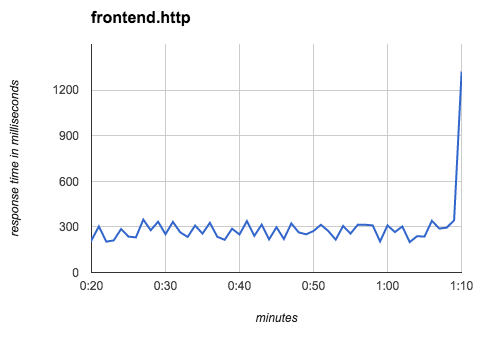
\includegraphics[scale=.6]{assets/frontend_http.png}
Brian (1:15): Something broken for sure, notification should be sent
Brian (1:17): hubot status yellow for frontend 
hubot (1:17): \emph{Status has been set to yellow and team has been notified}
Brian (1:18): Let's see who deployed last time, they rolled 
              out something new
Brian (1:18): hubot deploy frontend
hubot (1:18): Last deploy for frontend was 2 days
Brian (1:18): Nothing happened here, so no new code,
              but something is broken, interesting
Brian (1:24): hubot graph frontend.exception-rate @-1h
....
hubot (3:00): \emph{Oncall rotation has been changed}
hubot (3:00): \emph{Incident 1337 is still active, 
              @Simon has been notified}
Simon (3:00): Popping in, @Brian you can get some sleep
Brian (3:00): Thanks @Simon, I tried my best, the error is still on
  \end{alltt}
  \caption[DUMMY]%
  {Incidens kezelés ChatOps használatával}%
  \label{lst:oncall_message}
\end{figure}

\Aref{lst:oncall_message} beszélgetés jól szemlélteti, hogy a chat segítségével mennyivel könnyebben végre lehet hajtani az elvégzendő a feladatokat.\\
\begin{itemize}
  \item Az értesítés kiküldése után, az incidens kezelése már a robot segítségével elvégezhető.
  \item Az információ összegyűjtése és a metrikák könnyen elérhetőek, mert a grafikonok és a legutóbbi élesítés dátuma lekérdezhetőek egyszerűen chaten keresztül.
  \item A felelős csapat értesítése és a státuszoldal frissítése is a korábban bemutatott módon elvégezhető.
  \item Minden lépés dokumentálva van, ugyanis minden beírt parancs látható mindenki számára (és naplózásra kerül).
  \item A Runbook utasításainak követése is megoldható a robot segítségével, vagy akár a kereső használatával könnyen kideríthető, hogy volt-e már korábban ilyen probléma akár ennél az alkalmazásnál vagy másiknál. Amennyiben volt, az ott használt parancsok használatával is el lehet kezdeni a hibajavítást.
  \item A hiba meg nem javítása esetén nem szükséges felvilágosítani a következő ügyelest, ugyanis az előzmények megtekintésével gyorsan világossá válhat számára is, hogy milyen műveletek lettek végrehajtva a hiba megjelenése óta.
\end{itemize}

Ahhoz, hogy az incidens menedzsment ennyire automatizáltan tudjon működni és ki lehessen használni a chat javára felsorolt előnyöket, erős szervezeti támogatottságra van szükség, és a chaten található adatokat kell használni, mint az információ egyetlen forrását. Ezen felül minden rendszernek (incidens menedzsment szoftver, monitorozó rendszer, metrika/napló rendszer) rendelkeznie kell programozható interfésszel, melyen keresztül a robot képes az információkhoz való hozzáférést biztosítani.\\
Ebben a részben nem került tárgyalásra, de mindennek a működéséhez szükséges, hogy az alkalmazásokból a megfelelő metrikák beküldésre kerüljenek, a hibák a központi naplózó rendszerbe bekerülnek, a monitorozható végpontok nem fals negatív adatokat szolgáltatnak. Ezeknek a megfelelő működése a fejlesztési csapat felelőssége.

\chapter{A szervezeti integráció}
%!TEX root = ./dolgozat.tex

\section{Áttekintés}
\label{sect:futureops_overview}
Ahhoz, hogy egy szolgáltatás vagy egy alkalmazás (hosszú távon) működtethető legyen az előző fejezetekben bemutatásra kerültek a szükséges részek.

\begin{description}
  \label{dsc:important_stuffs}
  \item[Folyamatos adatgyűjtés és értesítés]\hfill\\
  Az alkalmazás és a környezetének adatainak és metrikáinak folyamatos gyűjtése, a jó és a jól működésre való törekedés végett.
  \item[Gyűjtött adatok elemzése]\hfill\\
  A nagymennyiségű adatgyűjtés miatt, a zaj csökkentése érdekében cselekvésre sarkalló elemzésre és kimutatásokra van szükség.
  \item[Automatizált folyamatok]\hfill\\
  Az automatizálás segítségével a hibák száma minimalizálható, a feladatok újra és újra megismételhetőek, hordozhatókká, újrafelhasználható válnak növelve a tudásmegosztást.
  \item[A rendszerek közti kapcsolatok megértése]\hfill\\
  A szoftverfejlesztési látókör kibővítése, a működtetéshez szükséges környezet való hozzáférés csökkenti a reakcióidőt, a szakmai döntésekhez szükséges idő rövidül, gördülékenyebb lesz.
  \item[Transzparens kommunikáció]\hfill\\
  Transzparens kommunikáció, melynek segítségével a szervezet tagjai közvetlenül és azonnal elérhetőek, reszponzívabb eszmecserét és visszakereshető kronológiai tudástárat eredményez.
\end{description}

{\Large A szervezet célja nem az, hogy mindenki értsen mindenhez hanem, hogy az egyénileg és csoportosan birtokolt tudás megosztása, minél egyszerűbb legyen és mindez minél kevesebb kontextusváltást igényeljen.\\}
\hfill\\
Amennyiben a szervezet a fenti listában szereplő elemeket implementálja, akkor rendkívül fontos, hogy az felsorolt adatok minél egyszerűbben elérhetőek legyenek. Az ehhez vezető legjobb mód, ha minden alkalmazás (dokumentáció-, verziókezelő rendszer) nem csak saját felülettel, hanem API-val is rendelkezik. Ennek a szemléletmódnak a fontosságát jelzi, hogy az Egyesült Királyság kormánya a programozható interfész fontosságát külön fejezetet taglalja a szolgáltatás kézikönyvében (\cite{uk_gov_build_api}). Minden az állam által, és az állam részére előállított szoftvernek meg kell felelnie a kézikönyvben lefektetett szabályoknak. Ennek köszönhetően az elosztottan tárolt adatok egy meghatározott része, integrálva egy központi helyre tud bekerülni. Azonban ez nem azt jelenti, hogy egy alkalmazás által nyújtott szolgáltatások a programozható interfész segítségével egy másik felületen is megvalósíthatóak legyenek, hanem:

\begin{itemize}
  \label{lst:invocing_important_points}
  \item más alkalmazásokkal való integráció elősegítése
  \item előzetes bepillantás lehetősége az adatokhoz
  \item a műveletek egy-egy fázisának kiszervezése
  \item a változásokról értesítés kiküldése
\end{itemize}

\begin{figure}[H]
  \begin{alltt}
\colorbox[gray]{0.85}{
\parbox{\textwidth}{\center{2015. 03. 04.}}
}
Emily: Hey @Gavin, last week we signed the contract with
       the MicroCompany Ltd. company.
       Have you set up their first invoice with due date 03.31?
Gavin: Good question.
Gavin: @hubot search invoice for microcompany
hubot: There are 2 matches for search "microcompany":
       \href{http://invoicing.com/invoice/32}{#32} is for MicroCompany with VOID status, 
       its due date is: 2013. 04. 02. (almost 2 years ago)
       \href{http://invoicing.com/invoice/33}{#33} is for MicroCompany with PAID status (USD 1300),
       its due date is: 2013. 04. 02. (almost 2 years ago)
Gavin: Oh it seems I haven't drafted the new one.
Gavin: @hubot invoice draft "MicroCompany Ltd." on 2015.03.31.
hubot: \href{http://invoicing.com/invoice/98}{#DR98} has been drafted for MicroCompany Ltd. with due date 2015.03.31.
\colorbox[gray]{0.85}{
\parbox{\textwidth}{\center{2015. 03. 31.}}
}
Accounting Software:
       There is one invoice which is dated for today:
       \href{http://invoicing.com/invoice/98}{#DR98} for MicroCompany Ltd. 
       created by @Gavin 27 days ago
Gavin: Oh almost slipped out of my mind, on it. cc @Emily
Accounting Software:
       Gavin added USD 1500 to \href{http://invoicing.com/invoice/98}{#98} and set status to AUTHORISED.
Emily: Thanks @Gavin.
Emily: Fyi @Gavin I've just sent #98 to microcompany
hubot: \href{http://invoicing.com/invoice/98}{#98} is an invoice in 
AUTHORISED state, with amount USD 1500, its due date is 2015.03.31.
  \end{alltt}
  \caption[DUMMY]%
  {Szolgáltatás integráció, kontextusváltás csökkentése, a feladat egy felületen keresztüli menedzselése}%
  \label{lst:invoicing_using_chat}
\end{figure}

A fejezet elején található lista pontjai kerültek szemléltetésre \aref{lst:invoicing_using_chat} példában, itt egy szándékosan nem technikai feladattal kerül bemutatásra, ugyanis egy szolgáltatás működtetéséhez nem csak technikai problémákkal kell megküzdeni, hanem sok kommunikáció során, az egyik vagy akár mindkét résztvevő nem a programkóddal közvetlenül érintkező ember.
A beszélgetés Emily kérdésével kezdődik, aki azt szeretné tudni Gavintől, hogy előkészítette-e a számlát a példában szereplő cégnek. Gavin fejből nem tudja, -viszont ahelyett, hogy megnyitná a számlázó programot,- azonnal a beszélgetésből ellenőrizni tudja, hogy a számla már meg lett-e írva (\emph{más alkalmazással való integráció elősegítése}). Érdemes megfigyelni, hogy a listázott számláknak nem csak az azonosító száma kerül kiírásra (amely kattintható linkként jelenik meg, tehát azonnal megtekinthető egy gombnyomással a számlázórendszerben), hanem tartalmazza a legfontosabb információkat is (\emph{előzetes bepillantás lehetősége az adatokhoz}).\hfill\\
Miután Gavin meggyőződik róla, hogy a számla nincs a rendszerben, anélkül hogy belépne a számlázó szoftverbe, a beszélgetésből közvetlenül, könnyen elkészítheti az új számla előzetes verzióját. Természetesen nem cél a számla teljes elkészítése, csak az elkezdése, hiszen így a létrejövő piszkozati számlára már lehet hivatkozni a visszakapott azonosítóval (a műveletek egy-egy fázisának kiszervezése).\hfill\\
Az idő előrehaladtával, amikor a számla esedékessége közeledik, a számlázó rendszer üzenetet küldve (például \aref{section:service_integration} fejezetben bemutatott webhook segítségével) tudja értesíteni, a felelősöket arról, hogy teendő van a számlával. Gavin ezt észlelve, a számla számára klikkelve, a számlázó szoftverbe belépve, a számlát be tudja fejezni. A számla elkészültéről ismét értesítés kerül küldésre, ezáltal tudatva a többi érintettel a számla állapotváltozását (\emph{a változásokról értesítés küldés}), mindezt valós időben.\hfill\\
Érdemes megjegyezni, hogy az érintettek közti kommunikációt nagyban tudja javítani, ha egy számlaszám vagy egy számla linkjének a beszélgetésben történő említésére a chatrendszer vagy éppen a robot automatikusan letölti az API-n keresztül a számlaszámhoz tartozó legfontosabb adatokat és megjeleníti azokat.\\
\hfill\\
Érdemes továbbá megfigyelni \aref{lst:invoicing_using_chat} példában, hogy miközben egy feladat elvégzésre került, a feladatban a többi érintett is folyamatosan értesülhetett az állapotról, így sokkal könnyen be tudnak csatlakozni a beszélgetésbe, meg lehet érteni a beszélgetés kontextusát, gyorsabban lehet reagálni egy-egy kérdésre.
Amennyiben a szervezeten belüli centralizált kommunikáció aszinkron módon zajlik, akkor a kontextusváltások nincsenek ráerőltetve a szervezeti tagokra, hiszen az aktuálisan végzett feladat befejezése után is meg tudják válaszolni a számukra feltett kérdéseket.
Végül, ha a központi kommunikációs csatornán keresztül kerülnek automatizálásra egy-egy feladat elvégzéséhez szükséges lépések, akkor az adatokhoz hozzáféréssel rendelkezők köre bővülhet, ezáltal csökkentve egy-egy feladat megoldásának idejét.
Természetesen ez nem azt jelenti, hogy a szervezeten belül bárki bármihez hozzáférhet, legyen az a számlázi rendszer, vagy a chatrendszer egy szobája, a szervezetnek meg kell határoznia az adatokhoz való hozzáférhetőséget, legyen az írási vagy olvasási jog, de a dolgozatnak nem célja ennek meghatározása, ugyanis ezek a szabályok mindig az adott szervezet kultúrájától, az adatok milyenségétől és az adott iparágtól is erősen függenek.

\section[Hatásai a szoftverműködésre]{Hatásai a szoftverműködésre%
  \sectionmark{Hatásai\\a szoftverműködésre}}
\sectionmark{Hatásai\\a szoftverműködésre}

\Aref{sect:futureops_overview} fejezetben áttekintésre került, hogy a szervezet által használt eszközök integrációja hogyan javíthatja a munkavégzés minőségét. A következőkben pedig megvizsgálásra kerül, hogy mire kell figyelni, egy szoftverműködés során, milyen lépések azok, amelyeket végre kell hajtani, hogy a szolgáltatás felhasználói számára a működtetés szinte láthatatlan legyen.

\brparagraph{Fejlesztési környezet}
A fejlesztés során \aref{chap:cont_int}. és \aref{chap:cont_not}. fejezetben bemutatott lépések a legfontosabbak, azaz az adott fejlesztőcsapat, a projektmenedzser, az egyéb belső érintettek folyamatos tájékoztatása és a visszacsatolás idejének csökkentése, többek között a következő folyamatok esetén.
\begin{description}
  \item[a kódátnézés (code review)]\hfill\\
  A kódátnézés a használt szoftverfejlesztési metodologikától függetlenül fontos szerepet kell, hogy kapjon a fejlesztés során, ezért mind az átnézésért felelős szakember értesítése, mind a kód megírásáért felelős programozó részéről az igény jelen van az egyszerűbb és a reszponzívabb kommunikációra. Ennek oka, hogy ugyanaz a kódrészlet újbóli megértése komoly erőforrásokat emészthet el, továbbá egyik szereplőnek sem jó, ha egy kód nem kerül beolvasztásra a főágba vagy esetleg csak hosszú idő elteltével kerül beolvasztásra.
  \item[a kódminőség javítása]\hfill\\
  A kódátnézés magas erőforrásigénye miatt (az átnézést végzőnek a minél jobb kódminőség elérése, a logikai hibák megtalálása a célja; a kód írójának pedig a saját munkája eredményének a megvédése a célja, ez gyakran szakmai vitához, egyet nem értéshez vezethet, amelynek feloldása hosszabb időt vehet igénybe) csökkenteni kell a kódátnézés iterációinak számát, ezért a kódminőség automatizált ellenőrzésével kizárhatóak azok a hibák (szintaktikai hibák, elérhetetlen kódrészletek), amelyek biztosan nem mennének át a kódátnézés folyamatán.
  \item[folyamatos tesztelés]\hfill\\
  A folyamatos tesztelés eredménye, amely automatizált tesztesetéknél a korábban megírt tesztek (egység, regressziós, integrációs) kimenetét és a hibás teszt azonosítóját elküldve értesíti a felelős egyént vagy csoportot. A folyamatos tesztelés másik típusa, a manuális tesztek, melyek érkezhetnek a minőségellenörző csapattól (QA) vagy egy az integrációt végző másik csapattól, ezért fontos, hogy a visszacsatolás minél egyszerűbben és gyorsabban megoldható legyen.
  \item[automatizálás]\hfill\\
  Az alkalmazáshoz kapcsoló feladatok közül, nem csak a produkciós környezetben kell az automatizálást komolyan venni, és aktívan használni, hanem már a fejlesztés során is. Automatizálás magába foglalhatja a konfiguráció menedzsmentet (amelyet szintén tesztelni kell, tehát igaz rá a fejlesztési környezet minden pontja), a tesztelést (egység, több környezetben is használható integrációs tesztek), performancia problémák detektálását.
\end{description}

\brparagraph{Élesítés}
Az élesítés az a folyamat, amely során a kód a fejlesztési környezetből a produkciós környezetbe kerül. A dolgozat nem különíti el a kódélesítést (deploy) és a funkcióélesítést (release), mert bár a legtöbb szoftver élesítésre ezek elkülönítésre kerülnek, azonban a felmerülő pontok, amelyekre figyelmet kell fordítani mindkét esetben ugyanúgy jelen vannak. Az élesítés során a legfontosabb lépések, amelyeket figyelembe kell venni a következők:
\begin{description}
  \item[Konfiguráció menedzsment]
  A konfiguráció menedzsmentről már esett szó a fejlesztési környezet pontjai között, viszont érdemes itt is kiemelni, mert klasszikusan ennél a lépésnél használják, viszont ha két helyen is használatra kerül, az azt jelenti, hogy mindenki magabiztosabban nyúl hozzá, sokkal több kézen fordul meg, sokkal több tapasztalattal fog rendelkezni a szervezet és sokkal kiforrottabbá fog válni a konfiguráció menedzsment.
  \item[Folyamatos integráció]
  A fejlesztési környezetnél már erről is szó esett, mégpedig az automatizált tesztek és a kódellenőrzés lépeseknél, bár ez így nem lett kijelentve. Tulajdonképpen a folyamatos integráció lépései a kódminőség ellenőrzésével, a tesztek futtatásával kezdődik, míg a fejlesztés során ezek után az eredmény kerül publikálásra, addig az élesítés során egy további plusz lépéssel a kód az éleskörnyezetbe fog kerülni.
  \item[Változáskövetés]
  A változáskövetést általában egy változás naplóban (changelog) végzik, amely egy projekt megemlítendő változásait tartalmazza válogatott és kronológiailag rendezett formában (\cite{keep_a_changelog}).
\end{description}

\brparagraph{Hibadetektálás}
A hibák detektálása az élesítés közben és után folyamatos feladatként jelentkezik, a hibák a beérkező adatfolyamokból kerülnek kalkulálásra, ezeknek két típusa van:
\begin{itemize}
  \item külső adatok
  \item belső adatok
\end{itemize}

A belső adatok az alkalmazás által küldött naplóbejegyzésekből és számosítható metrikákból épülnek fel.\\
A külső adatok független ellenőrzésekből, részben vagy teljesen harmadik fél által végzett vizsgálatokból állnak (működik-e az alkalmazás, alkalmazás válaszideje milliszekundumban, megfelelő válasz érkezik-e a kérésre), amelyek nincsenek kapcsolatban az aktuálisan ellenőrzött rendszerrel. Rendkívül fontos, hogy a hibák detektálása adaptív legyen, mind a környezetre, mind a rendszer aktuális állapotára. Néhány példa ennek szemléltetésére:

\begin{itemize}
  \item Egy alkalmazás sebessége függ a felhasználók számától, az aktuális időponttól (egy közösségi oldal életében este 6 és 8 óra között feltehetően magas lesz a felhasználók száma), az aktuális időjárástól (hideg, esős idő esetén nőhet a felhasználók száma), ezért eltérően kell tudni kezelni a kedd este 6 órát és a vasárnap hajnali 4 órát, mert míg az előbbi időpontban az alkalmazás válaszidejének növekedése mindössze az aktív felhasználók számának növekedését jelzi, addig az utóbbi esetben felhetehetően hiba okozza. Ezetén érdemes több metrika együttesét figyelembe venni, illetve időablakokat alkalmazni.
  \item Hibák közti priorizálás alkalmazása esetén, egy új hiba felbukkanása az ügyeleteseket nem szakítja meg a már korábban jelzett hiba felderítése, illetve megoldása közben. Ilyen lehet, ha egy adatközpont hálózati problémákkal küzd, akkor nem érdemes értesíteni mindenkit arról is (vagy esetleg alacsonyabb priorizálással), hogy az adott adatközpontban futó alkalmazások is leálltak.
  \item Akcióra kész hibák használata. Annak ellenére, hogy külső adatfolyamból érkező hibák érthetőek, ez nem azt jelenti, hogy az azokat követő hibajavítás is egyértelmű lenne vagy esetleg meghatározható lenne. Ezért a több forrásból érkező adatfolyamokat (külső ellenőrzés, alkalmazás naplóbejegyzései, konténer naplóbejegyzései, hiba előidézésében részt vevő egyéb komponensek naplóüzenetei, metrikái) összegyűjtésével megérthető a hibák a kontextusa, a későbbi ismételt előidézhetőség esélye megnő, szükség esetén (regressziós) tesztesettel lefedhetővé válik.
\end{itemize}

\brparagraph{Hibaelhárítás}
A hibaelhárítása a hiba detektálása után kezdődik el, melynek első lépése az incidens kezelő rendszerből érkező értesítés kezelése. Ezt követően a beérkező hibához kapcsolódó naplóüzenetek és elérhető grafikonok (hasonlóan, mint \aref{lst:oncall_message} példában látható) megtekintése, a hiba okának detektálása, majd az előzetes szabálygyűjtemény (runbook) alapján történő végrehajtás megkezdése.
Emellett publikus szolgáltatás vagy végfelhasználót is érintő probléma esetén erősen ajánlott a szolgáltatás státuszoldalát is frissíteni, hogy reflektálja a fennálló hiba létét, az érintett komponseket és a várható javítás idejét, amennyiben lehetséges ennek megbecslése. A hiba javítása akár újabb emberek, csoportok bevonását is igényelheti. Gyakran előfordul, hogy a incidens megoldása magának az alkalmazásnak a módosítását is igényli, amely ilyenkor ismét végigmegy az a fejlesztési környezet és az élesítés lépésein.\hfill\\
A hibajavítás befejeztével az incidens lezárásra kerül, a szolgáltatásért felelősök és  amennyiben szükséges az érintett felhasználók is értesítésre kerülnek.

\brparagraph{Hiba-utóélet}
Minden hiba után általában két-három nappal később érdemes egy úgynevezett post mortem analízist tartani. A nem közvetlenül az incidens lezárása után tartott analízis azért fontos, mert ilyenkor már a hibát övező érzelmek csökkennek (egy éjszaka három órakor érkező riasztás sok negatív érzelemmel fogja eltölteni az ügyeletest), viszont még nem került elfelejtésre a hiba oka és a javítás folyamata. A post mortem analízis egy írásos dokumentummal záródó megbeszélés, amely tartalmazza a hiba körülményeit, a megoldáshoz szükséges akciókat és a későbbi megelőzéshez szükséges lépéseket.\hfill\\
A modern szervezetekben gyakran alkalmazott metodológia a hibáztatásmentes post mortem (blamess post mortem), amely a hibák okozta szolgáltatáskieséseket a szervezet tanulási folyamataként látják, nem pedig a hibás személy kilétét próbálják meg felfedni és megbüntetni (\cite{blameless_post_mortem}).
A felelős személy meghatározása egy elosztott rendszerben szinte lehetetlen, ezért érdemes inkább a post mortem analízist egy tanulási lehetőségként értelmezni, mint a büntetés egy formájának tekinteni. Továbbá nagy skálázású alkalmazásoknál incidensek gyakran előfordulnak, ezért az üzemeltetőket érdemes támogatni abban, hogy nyíltan beszéljenek a post mortem alkalmával az általuk elvégzütt lépésekről, ezáltal csökkentve az incidensek okozta stresszt.

\chapter{Összefoglalás}
%!TEX root = /Users/oroce/Documents/msc-szakdolgozat/dolgozat.tex
A szoftverek működtetése komplex dolog, de az adatalapú szemlélettel magabiztosan lehet őket működtetni. A magasfokú automatizálással a szoftverek külső beavatkozás nélkül tesztelhetőek, ellenőrizhetőek így csökkentve a hibázási lehetőséget. Az újrafelhasználással a komplex rendszerek is lebonthatóak apró alkotóelemekre, melyeknek megértése sokkal könnyebb és gyorsabb monolitikus társaiknál. Ez a két alkotóelem, amely meghatározza egy alkalmazás működtethetőségét technikai oldalról.\hfill\\
A másik oldalon viszont a szervezet tagjai vannak és a köztük történő kommunikáció. Az ismétlődő folyamatok automatizálásával csökken a szervezet tagjai felé támasztott humánerőforrás igény, viszont a tervezésnél és a problémák megoldásánál nagyfokú kommunikációra és koordinációra van szükség. Ennek a problémának a megoldása lehet a chat alapú, szobákra osztott, csoportos kommunikáció, amely az aszinkronitásával, az eszköz- és helyfüggetlenségével nagyban hozzájárulhat a szervezetek egy egységes, központi és transzparens információcseréjéhez. Továbbá a központi chat lehet az a gócpontja a szervezetnek, ahová befutnak a külső forrásokból érkező adatok, ahol egy-egy üzenetre az akció azonnal végrehajtható kontextus váltás nélkül, növelve a szervezet tagjainak információellátottságát, megteremtve a tudásmegosztás platformját, mindezt visszakereshetően és bárki számára elérhetően. Az incidensek felbukkanásakor a valósidejű viszont aszinkron kommunikáció a legjobb megoldás lehet arra, hogy a felhasználók észrevétlenül tudják továbbra is használni a szoftvert, miközben az érintettek maximális információellátottság mellett próbálják megoldani a felmerült problémát. Ha az incidensmenedzsmentbe bevonásra kerülnek az üzemeltetőkön kívül a fejlesztők is, akkor a tudásuk keresztezének köszönhetően a problémák forrásának detektálása és a megoldás ideje rövidülhet illetve a hibák utóéletének követése és azok elemzése - amelyeknek a működtetés részét kell képezniük - sokkal proaktívabbá válhat, és ezt a tudást felhasználva a szervezet többet profitálhat, a felhasználók elégedettebbek lesznek.

 %a mind üzemeltetési és mind fejlesztői tudással rendelkező szakemberek. A hibák utóéletének követése, azok elemzése a működtetés részének kell válnia és proaktívan kell segíteni a további fejlesztéseket.

% Mivel szoftverek üzemeltetésében a kommunikáció

%A dolgozat bemutatta, hogy miként lehet a kommunikáció ezen formáját a szoftverüzemeltetés kontextusában használni. 

%A dolgozat bemutatta ennek a valósidőben történő akcióvégrehajtásnak az előnyét a szoftveres hibák menedzselésére, miként lehet a fejlesztők és az üzemeltetők tudásánák keresztezését a szervezet javára fordítani, kitérve arra, hogy a hibautóélet kézelésének igenis a szoftverrendszerek részévé kell válnia és proaktívan kell segíteni a további fejlesztéseket.


 %Továbbá a szöveges üzenetekkel történő akciók elvégzése robot segítségével, amely a kontextus váltás csökkentése 

%Míg a szoftverek építésének folyamat optimalizációja, a megfelelő szoftverfejlesztési metodológiák használata a figyelem középpontjában vannak, addig maguknak a szoftverek működtetése kevés figyelmet kap. 
%A dolgozat bemutatja a webes alkalmazásokra fókuszálva, hogy egy alkalmazás életútja során egészen a kód megírásától a tesztelésen, az élesítésen át a hibaelhárításig milyen lépéseket kell követni, az iparágban leggyakrabban használt eszközök segítségével. \hfill\\

%Majd bemutatásra kerül, hogy a felhasznált eszközök hogyan integrálhatóak egybe, miként tudja a szervezet kihasználni a központosított aszinkron kommunikáció előnyeit, csökkentve a kontextusváltások és a folyamatos megszakítások okozta stresszt. 

\newpage

\printbibliography

\end{document}

